%%%% Шаблон Отчета по практике <<SPbPU-student-thesis-template>>  %%%%
%%
%%   Создан на основе глубокой переработки шаблона российских кандидатских и докторских диссертаций [1]. 
%%   
%%   Полный список различий может быть получен командами git.
%%   Лист авторов-составителей расположен в README.md файле.
%%   Подробные инструкции по использованию в [1,2].
%%   
%%   Рекомендуем установить TeX Live + TeXstudio
%%   <<Стандартная>> компиляция 2-3 РАЗА с помощью pdflatex + biber (для библиографии)     
%%  
%%%% Student thesis template <<SPbPU-student-thesis-template>> %%%%
%%
%%   Created on the basis of deep modifification of the Russian candidate and doctorate thesis template [1]. 
%%   
%%   Full list of differences can be achieved by git commands.
%%   List of template authors can be seen in the README.md file.
%%   Detailed instructions of usage, see, please in [1,2].
%%     
%%   [1] github.com/AndreyAkinshin/Russian-Phd-LaTeX-Dissertation-Template 
%%   [2] Author_guide_SPBPU-student-thesis-template.pdf
%%   
%%   It is recommended to install TeX Live + TeXstudio   
%%   Default compilation 2-3 TIMES with pdflatex + biber (for the bibliography)
%%  
%%%% Preamble start %%%%  
%%
%%   Please, do not modify files in the preamble
%%
\newcommand*{\anyptfilebase}{template_settings/bpfont} 
\newcommand*{\anyptsize}{14} 		 
\RequirePackage[l2tabu,orthodox]{nag} 
\documentclass[extrafontsizes,a4paper,*pt,oneside,openany]{memoir}
%% Режим черновика
\makeatletter
\@ifundefined{c@draft}{
  \newcounter{draft}
  \setcounter{draft}{0}  % 0 --- чистовик (максимальное соблюдение ГОСТ)
                         % 1 --- черновик (отклонения от ГОСТ, но быстрая сборка итоговых PDF)
}{}
\makeatother

%% Библиография

%% Внимание! При использовании bibtex8 необходимо удалить все
%% цитирования из  ../common/characteristic.tex
\newcounter{bibliosel}
\setcounter{bibliosel}{1}           % 0 --- встроенная реализация с загрузкой файла через движок bibtex8; 1 --- реализация пакетом biblatex через движок biber

               
%%% Проверка используемого TeX-движка %%%
\usepackage{iftex}[2013/04/04]
\newif\ifxetexorluatex   % определяем новый условный оператор (http://tex.stackexchange.com/a/47579/79756)
\ifXeTeX
    \xetexorluatextrue
\else
    \ifLuaTeX
        \xetexorluatextrue
    \else
        \xetexorluatexfalse
    \fi
\fi

\RequirePackage{etoolbox}[2015/08/02]               % Для продвинутой проверки разных условий

%%% Поля и разметка страницы %%%

\usepackage{pdflscape}                              % Для включения альбомных страниц
\usepackage{geometry}                               % Для последующего задания полей

%%% Математические пакеты %%%
\usepackage{amsfonts,amsmath,amssymb,amscd,amsthm}  % Математические дополнения от AMS
% %amsthm should be loaded after amsmath!!

\usepackage{mathtools}                              % Добавляет окружение multlined

%%%% Установки для размера шрифта 14 pt %%%%
%% Формирование переменных и констант для сравнения (один раз для всех подключаемых файлов)%%
%% должно располагаться до вызова пакета fontspec или polyglossia, потому что они сбивают его работу
\newlength{\curtextsize}
\newlength{\bigtextsize}
\setlength{\bigtextsize}{13.9pt}

\makeatletter
%\show\f@size                                       % неплохо для отслеживания, но вызывает стопорение процесса, если документ компилируется без команды  -interaction=nonstopmode 
\setlength{\curtextsize}{\f@size pt}
\makeatother

%%% Кодировки и шрифты %%%
\ifxetexorluatex
    \usepackage{polyglossia}[2014/05/21]            % Поддержка многоязычности (fontspec подгружается автоматически)
\else
    \RequirePDFTeX                                  % tests for PDFTEX use and throws an error if a different engine is being used
   %%% Решение проблемы копирования текста в буфер кракозябрами
%    \input glyphtounicode.tex
%    \input glyphtounicode-cmr.tex %from pdfx package
%    \pdfgentounicode=1
    \usepackage{cmap}                               % Улучшенный поиск русских слов в полученном pdf-файле
    \defaulthyphenchar=127                          % Если стоит до fontenc, то переносы не впишутся в выделяемый текст при копировании его в буфер обмена
    
%    \usepackage[T2A]{fontenc}                       % Поддержка русских букв
    \usepackage[T2A,T1]{fontenc}
    \usepackage[utf8]{inputenc}[2014/04/30]         % Кодировка utf8
    \usepackage[english, russian]{babel}[2014/03/24]% Языки: русский, английский
\fi
\usepackage{tempora} %TemporaLGCUni of Times type
\usepackage{newtxmath} %math font of Times type
% need to set the monospace=typewritter font
%https://tex.stackexchange.com/questions/213835/using-many-typewriter-fonts-in-a-single-document

\makeatletter %load fonts for cmtt
\providecommand{\EC@ttfamily}[5]{%
	\DeclareFontShape{#1}{#2}{#3}{#4}{
		<-8.5>#50800
		<8.5-9.5>#50900
		<9.5-10.5>#51000
		<10.5-11.5>#51095
		<11.5-13>#51200
		<13-15.5>#51440
		<15.5-18.5>#51728
		<18.5-22>#52074
		<22-27>#52488
		<27-32>#52986
		<32->#53583}{}}
\DeclareFontFamily{T1}{cmtt}{}
\DeclareFontFamily{T2A}{cmtt}{}
\EC@ttfamily{T1}{cmtt}{m}{n}{ectt}
\EC@ttfamily{T1}{cmtt}{m}{sl}{ecst}
\EC@ttfamily{T1}{cmtt}{m}{it}{ecit}
\EC@ttfamily{T1}{cmtt}{m}{sc}{ectc}
\DeclareFontShape{T1}{cmtt}{bx}{n}%
{<->ssub*cmtt/m/n}{}
\DeclareFontShape{T1}{cmtt}{bx}{it}%
{<->ssub*cmtt/m/it}{}
\EC@ttfamily{T2A}{cmtt}{m}{n}{latt}
\EC@ttfamily{T2A}{cmtt}{m}{sl}{last}
\EC@ttfamily{T2A}{cmtt}{m}{it}{lait}
\EC@ttfamily{T2A}{cmtt}{m}{sc}{latc}
\DeclareFontShape{T2A}{cmtt}{bx}{n}%
{<->ssub*cmtt/m/n}{}
\DeclareFontShape{T2A}{cmtt}{bx}{it}%
{<->ssub*cmtt/m/it}{}
\makeatletter

%\makeatletter %load fonts for cmtt
%\providecommand{\EC@ttfamily}[5]{%
%	\DeclareFontShape{#1}{#2}{#3}{#4}{
%		<-8.5>#50800
%		<8.5-9.5>#50900
%		<9.5-10.5>#51000
%		<10.5-11.5>#51095
%		<11.5-13>#51200
%		<13-15.5>#51440
%		<15.5-18.5>#51728
%		<18.5-22>#52074
%		<22-27>#52488
%		<27-32>#52986
%		<32->#53583}{}}
%\DeclareFontFamily{T2A}{cmtt}{\hyphenchar\font\m@ne}
%\EC@ttfamily{T2A}{cmtt}{m}{n}{latt}
%\EC@ttfamily{T2A}{cmtt}{m}{sl}{last}
%\EC@ttfamily{T2A}{cmtt}{m}{it}{lait}
%\EC@ttfamily{T2A}{cmtt}{m}{sc}{latc}
%\DeclareFontShape{T2A}{cmtt}{bx}{n}%
%{<->ssub*cmtt/m/n}{}
%\DeclareFontShape{T2A}{cmtt}{bx}{it}%
%{<->ssub*cmtt/m/it}{}
%\makeatletter

%\makeatletter
%\input{t1lmtt.fd}
%\@namedef{T1+lmtt}{}
%\makeatother


\renewcommand{\ttdefault}{cmtt}
%\renewcommand{\ttdefault}{lcmtt} %покрупнее
%\usepackage[scaled=.85]{DejaVuSansMono} %слишком похож на рубленый
%\newfont{\wasyten}{wasy10} %название команды для вызова / название шрифта



%Другие шрифты:
% математика
%\usepackage[lite]{mtpro2}
%https://pctex.com/mtpro2.html
% текст        
% https://www.ctan.org/pkg/paratype
%       \usepackage[scaled=0.925]{XCharter}[2017/06/25] % Подключение русифицированных шрифтов XCharter
%\usepackage{pscyr}
%    \IfFileExists{pscyr.sty}{}{}  % Красивые русские шрифты
%\fi

%https://tex.stackexchange.com/questions/8260/what-are-the-various-units-ex-em-in-pt-bp-dd-pc-expressed-in-mm
\usepackage{printlen} %для измерения и вывода параменторов шрифтов, отступов, интервалов

\usepackage{bm} %для жирных начертаний символов

\usepackage{csquotes} %to check quotes

%%% Оформление абзацев %%%
\usepackage{indentfirst}                            % Красная строка

%%% Цвета %%%
%\usepackage[dvipsnames,usenames]{color}
\usepackage{colortbl}
\usepackage[dvipsnames, table, hyperref, cmyk]{xcolor} % Вероятно, более новый вариант, вместо предыдущих двух строк. Конвертация всех цветов в cmyk заложена как удовлетворение возможного требования типографий. Возможно конвертирование и в rgb.

%%% Таблицы %%%
\usepackage{longtable}                              % Длинные таблицы
\usepackage{multirow,makecell}                      % Улучшенное форматирование таблиц:
													% multirow - строки на несколько ячеек, 
												
													% makecell - сесколько строк в ячейке.
													% не работает, если внутри, например, \verb|text| -> \texttt{text}
													% аналоги
%https://tex.stackexchange.com/questions/2441/how-to-add-a-forced-line-break-inside-a-table-cell								
						
													

%%% Общее форматирование
%\usepackage{soul} % используется ulem
\usepackage{soulutf8}                               % Поддержка переносоустойчивых подчёркиваний и зачёркиваний
\usepackage{icomma}                                 % Запятая в десятичных дробях



%%% Предметный указатель  ГОСТ 7.78-99 Index %%%
%c обобщенными рубриками или развернутый
%или указатель терминов (в общем случае - произвольное число указателей)
%подключать до hyperref

%\usepackage{makeidx} %возможно, необходимо подключить И/ИЛИ пройти Tools-> Commands -> MakeIndex

\usepackage{imakeidx} 
%\indexsetup{level=\section*,toclevel=section,noclearpage}
\makeindex[program=makeindex,
options=-s template_settings/common/myindex.ist, %подключаем стилевой файл для форматирования вывода
name=ru, % префикс для русских указателей 
% если убрать <<ru>>, то для работы дефолтового придется вручную включать Tools-> Commands -> MakeIndex
title={\chapterLight{} 
%   \hrule{}
	Предметный указатель
%	\hrule{}
} 
%,columns=1 %по умолчанию 2
]
\makeindex[program=makeindex,
options=-s template_settings/common/myindex.ist, %подключаем стилевой файл для форматирования вывода
name=en, % префикс для английских указателей
title={\chapterLight{}
%	\hrule{}
	Index
%	\hrule{}
} 
%,columns=1 %по умолчанию 2
] 
%убрать добавление <<title>> в содержание:
%\noindexintoc %not to add index title in PURE makeidx %intoc is false by default with imakeidx


%       https://tex.stackexchange.com/a/132415/44348
%\makeatletter
%% we want hyphenation also in the first word
\renewcommand{\@idxitem}{\par\hangindent40\p@\hspace{0pt}\ignorespaces}
%% we don't want a page break before a subitem %implemented in the previous one
%%\renewcommand\subitem{\@idxitem\nobreak\hspace*{20\p@}}
%\makeatother


%%% Фиксация плавающих объектов





%%% Гиперссылки %%%
\usepackage{hyperref}[2012/11/06]

%%% Изображения %%%
\usepackage{graphicx}[2014/04/25]                   % Подключаем пакет работы с графикой

%%% Списки %%%
\usepackage[shortlabels]{enumitem} % shortlabels для того, чтобы изменять токены в списках с дефолтных (иерархическая структура) на произвольныею

%%% Подписи %%%
\usepackage{caption}[2013/05/02]                    % Для управления подписями (рисунков и таблиц) % Может управлять номерами рисунков и таблиц с caption %Иногда может управлять заголовками в списках рисунков и таблиц


\usepackage{subcaption}[2013/02/03]                 % Работа с подрисунками и подобным

%%% Счётчики %%%
%\usepackage[figure,table]{totalcount}               % Счётчик рисунков и таблиц. Взамен используется xassoccnt 
\usepackage{totcount}                               % Пакет создания счётчиков на основе последнего номера подсчитываемого элемента (может требовать дважды компилировать документ)
\usepackage{totpages}                               % Счётчик страниц, совместимый с hyperref (ссылается на номер последней страницы). Желательно ставить последним пакетом в преамбуле

\usepackage{xassoccnt} % для подсчета сумм приложений, рисунков, таблиц 


%%% Продвинутое управление групповыми ссылками (пока только формулами) %%%
\ifxetexorluatex
    \usepackage{cleveref}                           % cleveref корректно считывает язык из настроек polyglossia
\else
    \usepackage[russian]{cleveref}                  % cleveref имеет сложности со считыванием языка из babel. Такое решение русификации вывода выбрано вместо определения в documentclass из опасности что-то лишнее передать во все остальные пакеты, включая библиографию.
\fi
\creflabelformat{equation}{#2#1#3}                  % Формат по умолчанию ставил круглые скобки вокруг каждого номера ссылки, теперь просто номера ссылок без какого-либо дополнительного оформления



\ifnumequal{\value{draft}}{1}{% Черновик
    \usepackage[firstpage]{draftwatermark}
    \SetWatermarkText{DRAFT}
    \SetWatermarkFontSize{14pt}
    \SetWatermarkScale{15}
    \SetWatermarkAngle{45}
}{}

  
\input{template_settings/Dissertation/dispackages}         
\input{template_settings/Dissertation/userpackages}         
%% Режим черновика
\makeatletter
\@ifundefined{c@draft}{
  \newcounter{draft}
  \setcounter{draft}{0}  % 0 --- чистовик (максимальное соблюдение ГОСТ)
                         % 1 --- черновик (отклонения от ГОСТ, но быстрая сборка итоговых PDF)
}{}
\makeatother

%% Библиография

%% Внимание! При использовании bibtex8 необходимо удалить все
%% цитирования из  ../common/characteristic.tex
\newcounter{bibliosel}
\setcounter{bibliosel}{1}           % 0 --- встроенная реализация с загрузкой файла через движок bibtex8; 1 --- реализация пакетом biblatex через движок biber

               
\input{template_settings/Dissertation/preamblenames}       
%%% Кодировки и шрифты %%%
\ifxetexorluatex
    \setmainlanguage[babelshorthands=true]{russian}  % Язык по-умолчанию русский с поддержкой приятных команд пакета babel
    \setotherlanguage{english}                       % Дополнительный язык = английский (в американской вариации по-умолчанию)
    \setmonofont{Courier New}
    \newfontfamily\cyrillicfonttt{Courier New}
    \ifXeTeX
        \defaultfontfeatures{Ligatures=TeX,Mapping=tex-text}
    \else
        \defaultfontfeatures{Ligatures=TeX}
    \fi
    \setmainfont{Times New Roman}
    \newfontfamily\cyrillicfont{Times New Roman}
    \setsansfont{Arial}
    \newfontfamily\cyrillicfontsf{Arial}
\else
    \IfFileExists{pscyr.sty}{\renewcommand{\rmdefault}{ftm}}{}
\fi

%%% Подписи %%%
\captionsetup{%
singlelinecheck=off,                % Многострочные подписи, например у таблиц
skip=5pt,                           % Вертикальная отбивка между подписью и содержимым рисунка или таблицы определяется ключом
justification=centering            % Центрирование подписей, заданных командой \caption
}

%\setlength{\abovecaptionskip}{0pt} %альтернатива для skip, но не распространяется на longtable!
%\setlength{\belowcaptionskip}{0pt}
%\captionwidth{\linewidth}
%\normalcaptionwidth

% для изменения отступов от floats (e.g. table,figure) & minipage
\newlength{\mfloatsep}
\setlength{\mfloatsep}{4mm plus 0.7mm minus 0.7mm} %3mm для A5

% фиксируем расстояния с помощью пакета layouts
\setlength{\textfloatsep}{\mfloatsep} % расстояние от текста до float, если float прижат к верхнему или нижнему краю
\setlength{\floatsep}{\mfloatsep} % расстояние от float до float (если оба сверху/снизу)
\setlength{\intextsep}{\mfloatsep} % расстояние от текста до float, если float снизу и сверху ограничен текстом 
%
%% фактически из-за бокса, внутрь которого помещается \captionof{figure} происходит увеличаение на 1мм отступа в соответствующем элементе!
%
%% по требованиям СПбПУ как раз необходим отступ 4мм от рисунка


%Возможно более гибко задавать отступы, например:
%\setlength{\floatsep}{12pt plus 2pt minus 2pt}
%\setlength{\textfloatsep}{20pt plus 2pt minus 4pt}
%\setlength{\intextsep}{\floatsep}

%https://tex.stackexchange.com/questions/60477/remove-space-after-figure-and-before-text
%https://tex.stackexchange.com/questions/26521/how-to-change-the-spacing-between-figures-tables-and-text




%%% Парный к \smallA шрифт 13bp в подписи%%%
%TO-DO как напрямую связать со \smallA
%\DeclareCaptionFont{font13bp}{\smallA\selectfont} %к сожалению, приводит к отсупу после номера рисунка
\DeclareCaptionFont{font13bp}{\fontsize{13bp}{16.77bp}\selectfont} %аналог задания вручную
\DeclareCaptionFont{font12bp}{\small\selectfont} %аналог задания вручную



%%% Рисунки %%%
\DeclareCaptionLabelSeparator*{emdash}{~--- }             % (ГОСТ 2.105, 4.3.1)

\DeclareCaptionLabelFormat{figwithoutspace}{#1#2}
%\captionsetup[figure]{labelformat=figwithoutspace,labelsep=none,name=Fig.}

\captionsetup[figure]{labelformat=figwithoutspace,labelsep=\figlabelsep,position=bottom,labelfont={font12bp},textfont={font12bp}}

%\setlength{\belowcaptionskip}{0pt} %расстояние между 
%\caption* -- подрисуночной подписи и
%\caption  -- подписи к рисунку с номером
%необходимо менять вслед за добавлением \vskip в \captionsetup

%\setfloatadjustment{figure}{%
%	\setlength{\belowcaptionskip}{-3pt}   % чтобы обивка после рисунков была 3mm, так как caption добавляет около 1мм к 3мм. 
%}




%%% Таблицы %%%
\ifnumequal{\value{tabcap}}{0}{%
    \newcommand{\tabcapalign}{\raggedright}  % по левому краю страницы или аналога parbox

    \DeclareCaptionFormat{tablecaption}{\tabcapalign #1#2#3}
    \captionsetup[table]{labelsep=emdash}        % тире как разделитель идентификатора с номером от наименования
}{%
    \ifnumequal{\value{tablaba}}{0}{%
        \newcommand{\tabcapalign}{\raggedright}  % по левому краю страницы или аналога parbox
    }{}

    \ifnumequal{\value{tablaba}}{1}{%
        \newcommand{\tabcapalign}{\centering}    % по центру страницы или аналога parbox
    }{}

    \ifnumequal{\value{tablaba}}{2}{%
        \newcommand{\tabcapalign}{\raggedleft}   % по правому краю страницы или аналога parbox
    }{}

    \ifnumequal{\value{tabtita}}{0}{%
        \newcommand{\tabtitalign}{\raggedright}  % по левому краю страницы или аналога parbox
    }{}

    \ifnumequal{\value{tabtita}}{1}{%
        \newcommand{\tabtitalign}{\centering}    % по центру страницы или аналога parbox
    }{}

    \ifnumequal{\value{tabtita}}{2}{%
        \newcommand{\tabtitalign}{\raggedleft}   % по правому краю страницы или аналога parbox
    }{}

    \DeclareCaptionFormat{tablecaption}{\tabcapalign #1#2\par %\hline  % Идентификатор таблицы на отдельной строке
        \tabtitalign{#3}}                                       % Наименование таблицы строкой ниже
    \captionsetup[table]{labelsep=\tablabelsep}                 % разделитель идентификатора с номером от наименования
}
\DeclareCaptionFormat{tablenocaption}{\tabcapalign #1\strut}    % Наименование таблицы отсутствует

\newlength{\ltskip}
\setlength{\ltskip}{2pt}
\captionsetup[table]{format=tablecaption,singlelinecheck=off,position=top,labelfont={font12bp},textfont={font12bp}}  % многострочные наименования и прочее
\DeclareCaptionLabelFormat{continued}{\\[-14pt]Продолжение табл.~\!#2}



%%% Подписи подрисунков %%%
\renewcommand{\thesubfigure}{\alph{subfigure}}           % Буквенные номера подрисунков
\captionsetup[subfigure]{font={font12bp},               % Шрифт подписи названий подрисунков (отличается от основного)
	labelfont={font12bp},textfont={font12bp},
    labelformat=brace,                                    % Формат обозначения подрисунка
    singlelinecheck=off,
%    position=left,
    justification=raggedright 							 %выравнивание влево
%    justification=centering,                              % Выключка подписей (форматирование), один из вариантов            
}

%%% Подписи подрисунков SPbPU%%%
% реализован подход по первой ссылке, он позволяет масштабировать количество подрисунков
%https://tex.stackexchange.com/a/273169/44348
%https://tex.stackexchange.com/a/225914/44348
\usepackage[export]{adjustbox}



%%% Настройки гиперссылок %%%
\ifLuaTeX
    \hypersetup{
        unicode,                % Unicode encoded PDF strings
    }
\fi


\newcommand{\thesisTitle}{Название выпускной квалификационной работы}


\hypersetup{
    linktocpage=true,           % ссылки с номера страницы в оглавлении, списке таблиц и списке рисунков
%    linktoc=all,                % both the section and page part are links
%    pdfpagelabels=false,        % set PDF page labels (true|false)
    plainpages=false,           % Forces page anchors to be named by the Arabic form  of the page number, rather than the formatted form
    %colorlinks,                 % ссылки отображаются раскрашенным текстом, а не раскрашенным прямоугольником, вокруг текста
    citebordercolor={0.287 0.89 0.349}, %(RGB colour) with default {0 1 0}: The colour of the box around citations
    filebordercolor={0 .5 .5}, % (RGB colour) with default {0 .5 .5}: The colour of the box around links to files
    linkbordercolor={0.93 0 0}, % (RGB colour) with default {1 0 0}: The colour of the box around normal links
    menubordercolor={1 0 0}, % (RGB colour) with default {1 0 0}: The colour of the box around Acrobat menu links
    urlbordercolor={0.313 0.776 0.878}, % (RGB colour) with default {0 1 1}: The colour of the box around links to URLs
    pdfborder={0 0 1}, % The style of box around links; defaults to a box with lines of 1pt thickness, but the colorlinks option resets it to produce no border.
%    linkcolor={linkcolor},
%    citecolor={citecolor},      % цвет ссылок-цитат
%    urlcolor={urlcolor},        % цвет гиперссылок
    %hidelinks,                  % Hide links (removing color and border)
%    pdftitle={\thesisTitle},    % Заголовок pdf-файла
%    pdfauthor={\AuthorFull},  % Автор
%    pdfsubject={\thesisSpecialtyNumber\ \thesisSpecialtyTitle},      % Тема
%    pdfcreator={Создатель},     % Создатель, Приложение
%    pdfproducer={Производитель},% Производитель, Производитель PDF
%    pdfkeywords={\keywords},    % Ключевые слова
    pdflang={eng}, %eng %ru
    % % bookmarks settings
    bookmarks=true,
    bookmarksnumbered=true, % put section numbers
    bookmarksopen=true, %open when the pdf is opened
    bookmarksopenlevel=0, %chapter's level is enough to see
    bookmarksdepth=0 %set the depth of the levels in the pdf navigation bar
}

% %improve the bookmarksnumbered representation:
\makeatletter
\renewcommand{\Hy@numberline}[1]{#1. } %add the dot after a number
\makeatother


\ifnumequal{\value{draft}}{1}{% Черновик
    \hypersetup{
        draft,
    }
}{}

%%% Шаблон %%%
\DeclareRobustCommand{\todo}{\textcolor{red}}       % решаем проблему превращения названия цвета в результате \MakeUppercase, http://tex.stackexchange.com/a/187930/79756 , \DeclareRobustCommand protects \todo from expanding inside \MakeUppercase
\AtBeginDocument{%
    \setlength{\parindent}{2.5em}                   % Абзацный отступ. Должен быть одинаковым по всему тексту и равен пяти знакам (ГОСТ Р 7.0.11-2011, 5.3.7).
}

%%% Списки %%%
% Используем короткое тире (endash) для ненумерованных списков (ГОСТ 2.105-95, пункт 4.1.7, требует дефиса, но так лучше смотрится)
\renewcommand{\labelitemi}{\normalfont\bfseries{--}}

%% Перечисление строчными буквами латинского алфавита (ГОСТ 2.105-95, 4.1.7)
\renewcommand{\theenumi}{\Alph{enumi}} % первый уровень иерархии %латинскийалфавит заглавные
\renewcommand{\labelenumi}{\theenumi.} 
%\renewcommand{\theenumii}{\alph{enumii}} % второй уровень иерархии %латинскийалфавит
%\renewcommand{\labelenumii}{\theenumii)} 
%
%
%% Перечисление строчными буквами русского алфавита (ГОСТ 2.105-95, 4.1.7)
\makeatletter
\AddEnumerateCounter{\asbuk}{\russian@alph}{щ}      % Управляем списками/перечислениями через пакет enumitem, а он 'не знает' про asbuk, потому 'учим' его
\makeatother
%%\renewcommand{\theenumi}{\asbuk{enumi}} %первый уровень нумерации
%%\renewcommand{\labelenumi}{\theenumi)} %первый уровень нумерации 
%%\renewcommand{\theenumii}{\asbuk{enumii}} %второй уровень нумерации
%%\renewcommand{\labelenumii}{\theenumii)} %второй уровень нумерации 
\renewcommand{\theenumii}{\arabic{enumii}} %второй уровень нумерации %арабские цифры
\renewcommand{\labelenumii}{\theenumii.} %второй уровень нумерации 
%\renewcommand{\theenumi}{\arabic{enumi}} %первый уровень нумерации %арабские цифры
%\renewcommand{\labelenumi}{\theenumi)} %первый уровень нумерации 
%
%\renewcommand{\theenumiii}{\asbuk{enumiii}} %третий уровень нумерации %русский алфавит
\renewcommand{\theenumiii}{\alph{enumiii}} %третий уровень нумерации %английский алфавит
\renewcommand{\labelenumiii}{\theenumiii)} %третий уровень нумерации 
%\renewcommand{\theenumiii}{\arabic{enumiii}} %третий уровень нумерации %арабские цифры
%\renewcommand{\labelenumiii}{\theenumiii)} %третий уровень нумерации 



\setlist{nosep,%                                    % Единый стиль для всех списков (пакет enumitem), без дополнительных интервалов.
    labelindent=\parindent,leftmargin=*%            % Каждый пункт, подпункт и перечисление записывают с абзацного отступа (ГОСТ 2.105-95, 4.1.8)
}



% asm packages required! In particular amsthm
%http://tex.stackexchange.com/questions/37472/spacing-before-and-after-with-newtheoremstyle

%theoremstyle{}
%plain : italic text, extra space above and below;
%definition : upright text, extra space above and below;
%remark : upright text, no extra space above or below.

\newtheoremstyle{myplain} %
{0} %space above
{0} %space below
{\itshape}
{\parindent}
{\bfseries}
{.}
{.5em}
{}

\newtheoremstyle{mydefinition} %
{0} %space above
{0} %space below
{}
{\parindent}
{\bfseries}
{.}
{.5em}
{}

\theoremstyle{myplain} %improved plain style
\newtheorem{m-theorem}{Теорема}[chapter] % reset theorem numbering for each chapter
\newtheorem{m-corollary}{Следствие}[chapter] % definition numbers are 
\newtheorem{m-proposition}{Утверждение}[chapter] % definition numbers are dependent on theorem numbers
\newtheorem{m-lemma}{Лемма}[chapter]
\newtheorem{m-axiom}{Аксиома}[chapter]

\theoremstyle{mydefinition} %improved definition style
\newtheorem{m-example}{Пример}[chapter] % same for example numbers
\newtheorem{m-definition}{Определение}[chapter]  % definition numbers
\newtheorem{m-condition}{Условие}[chapter]
\newtheorem{m-problem}{Проблема}[chapter]
\newtheorem{m-exercise}{Упражнение}[chapter]
\newtheorem{m-question}{Вопрос}[chapter]
\newtheorem{m-hypothesis}{Гипотеза}[chapter]
\newtheorem{m-task}{Задание}[chapter]



%%control skip of thm, plain style - ANOTHER VARIANT
%%http://tex.stackexchange.com/questions/85400/how-to-change-space-around-theorem-environments
%\makeatletter
%\def\thm@space@setup{%
%	\thm@preskip=0cm %
%	%	\thm@preskip=0cm plus 0.2cm minus 0.2cm
%	\thm@postskip=0cm % or whatever, if you don't want them to be equal
%	%	\thm@postskip=\thm@preskip % or whatever, if you don't want them to be equal
%}
%\makeatother
    
\input{template_settings/Dissertation/disstyles}           
\input{template_settings/Dissertation/userstyles}          
%%% Библиография. Общие настройки для двух способов её подключения %%%


%%% Выбор реализации %%%
\ifnumequal{\value{bibliosel}}{0}{%
    %%% Реализация библиографии встроенными средствами посредством движка bibtex8 %%%

%%% Пакеты %%%
\usepackage{cite}                                   % Красивые ссылки на литературу


%%% Стили %%%
%\bibliographystyle{BibTeX-Styles/utf8gost71u}    % Оформляем библиографию по ГОСТ 7.1 (ГОСТ Р 7.0.11-2011, 5.6.7)
\bibliographystyle{BibTeX-Styles/ugost2008mod}    % Оформляем библиографию по ГОСТ 7.1 (ГОСТ Р 7.0.11-2011, 5.6.7)
%.bst

\makeatletter
\renewcommand{\@biblabel}[1]{#1.}   % Заменяем библиографию с квадратных скобок на точку
\makeatother
%% Управление отступами между записями
%% требует etoolbox 
%% http://tex.stackexchange.com/a/105642
%\patchcmd\thebibliography
% {\labelsep}
% {\labelsep\itemsep=5pt\parsep=0pt\relax}
% {}
% {\typeout{Couldn't patch the command}}

%%% Список литературы с красной строки (без висячего отступа) %%%
%\patchcmd{\thebibliography} %может потребовать включения пакета etoolbox
%  {\advance\leftmargin\labelsep}
%  {\leftmargin=0pt%
%   \setlength{\labelsep}{\widthof{\ }}% Управляет длиной отступа после точки
%   \itemindent=\parindent%
%   \addtolength{\itemindent}{\labelwidth}% Сдвигаем правее на величину номера с точкой
%   \advance\itemindent\labelsep%
%  }
%  {}{}

%%% Цитирование %%%
\renewcommand\citepunct{;\penalty\citepunctpenalty%
    \hskip.13emplus.1emminus.1em\relax}                % Разделение ; при перечислении ссылок (ГОСТ Р 7.0.5-2008)


%%% Создание команд для вывода списка литературы %%%
\newcommand*{\insertbibliofull}{
\bibliography{biblio/othercites,biblio/authorpapersVAK,biblio/authorpapers,biblio/authorconferences}         % Подключаем BibTeX-базы % После запятых не должно быть лишних пробелов — он "думает", что это тоже имя пути
}

\newcommand*{\insertbiblioauthor}{
\bibliography{biblio/authorpapersVAK,biblio/authorpapers,biblio/authorconferences}         % Подключаем BibTeX-базы % После запятых не должно быть лишних пробелов — он "думает", что это тоже имя пути
}

\newcommand*{\insertbiblioother}{
\bibliography{biblio/othercites}         % Подключаем BibTeX-базы
}


%% Счётчик использованных ссылок на литературу, обрабатывающий с учётом неоднократных ссылок
%% Требуется дважды компилировать, поскольку ему нужно считать актуальный внешний файл со списком литературы
\newtotcounter{citenum}
\def\oldcite{}
\let\oldcite=\bibcite
\def\bibcite{\stepcounter{citenum}\oldcite}
  % Встроенная реализация с загрузкой файла через движок bibtex8
}{
    %%% Реализация библиографии пакетами biblatex и biblatex-gost с использованием движка biber %%%

%\usepackage{csquotes} % biblatex рекомендует его подключать. Пакет для оформления сложных блоков цитирования.
%%% Загрузка пакета с основными настройками %%%
\ifnumequal{\value{draft}}{0}{% Чистовик
\usepackage[%
backend=biber,% движок
bibencoding=utf8,% кодировка bib файла
%sorting=none,% настройка сортировки списка литературы
style=gost-numeric,% стиль цитирования и библиографии (по ГОСТ)
%%style=gost-authoryear,% стиль цитирования и библиографии (по ГОСТ)
%%%% выставить следующую опцию <<babel>> и закомментировать <<language=english>> для достижения многоязычных ссылок
babel=other, %выставим для отображения разных языков
%%language=english,%только английский = \setlanguage{}; autobib получение языка из babel/polyglossia, default: autobib % если ставить autocite или auto, то цитаты в тексте с указанием страницы, получат указание страницы на языке оригинала
%%autolang=other,%other многоязычная библиография
%%clearlang=true,% внутренний сброс поля language, если он совпадает с языком из babel/polyglossia
defernumbers=true,% нумерация проставляется после двух компиляций, зато позволяет выцеплять библиографию по ключевым словам и нумеровать не из большего списка
sortcites=true,% сортировать номера затекстовых ссылок при цитировании (если в квадратных скобках несколько ссылок, то отображаться будут отсортированно, а не абы как)
doi=true,% Показывать или нет ссылки на DOI
isbn=false% Показывать или нет ISBN, ISSN, ISRN
]{biblatex}[2016/09/17]%
}{%Черновик
\usepackage[%
backend=biber,% движок
bibencoding=utf8,% кодировка bib файла
sorting=none,% настройка сортировки списка литературы
]{biblatex}[2016/09/17]%
}
%%TO-DO: продумать автозамену всех полей hyphenation на language



%%% Подключение файлов bib %%%
%\addbibresource[label=other]{biblio/othercites.bib}
%\addbibresource[label=vak]{biblio/authorpapersVAK.bib}
%\addbibresource[label=papers]{biblio/authorpapers.bib}
%\addbibresource[label=conf]{biblio/authorconferences.bib}



%http://tex.stackexchange.com/a/141831/79756
%There is a way to automatically map the language field to the langid field. The following lines in the preamble should be enough to do that.
%This command will copy the language field into the  field and will then delete the contents of the language field. The language field will only be deleted if it was successfully copied into the langid field.
\DeclareSourcemap{ %модификация bib файла перед тем, как им займётся biblatex 
    \maps{
    	%% SPbPU
    	%% https://tex.stackexchange.com/a/229505/44348
    	\map{% delete month
    		\step[fieldset=month, null]
    		\step[fieldsource=date,
    		match=\regexp{([0-9]{4})-[0-9]{2}(-[0-9]{2})*},
    		replace=\regexp{$1}$5] % <<$5>> only for syntax highlihgting in IDE
    	}
%    	\map{% set current urldate
%    	\step[fieldset=urldate, null]	
%		\step[fieldset=urldate,fieldvalue={\the\year-\the\month-\the\day}]
%    	} 
%		\map{% не отображаем поле ``Глава''
%			\step[fieldset=chapter, null]
%			\step[fieldset=editor, null]
%		}
%    	} 
		\map{% перекидываем значения полей hyphenation в поля langid, которыми пользуется biblatex
			\step[fieldsource=hyphenation, fieldset=langid, origfieldval, final]
		}
        \map{% перекидываем значения полей language в поля langid, которыми пользуется biblatex
            \step[fieldsource=language, fieldset=langid, origfieldval, final]
            \step[fieldset=language, null]
        }
%        \map[overwrite, refsection=0]{% стираем значения всех полей addendum
%            \perdatasource{biblio/authorpapersVAK.bib}
%            \perdatasource{biblio/authorpapers.bib}
%            \perdatasource{biblio/authorconferences.bib}
%            \step[fieldsource=addendum, final]
%            \step[fieldset=addendum, null] %чтобы избавиться от информации об объёме авторских статей, в отличие от автореферата
%        }
        \map{% перекидываем значения полей numpages в поля pagetotal, которыми пользуется biblatex
            \step[fieldsource=numpages, fieldset=pagetotal, origfieldval, final]
            \step[fieldset=pagestotal, null]
        }
        \map{% если в поле medium написано "Электронный ресурс", то устанавливаем поле media, которым пользуется biblatex, в значение eresource.
            \step[fieldsource=medium,
            match=\regexp{Электронный\s+ресурс},
            final]
            \step[fieldset=media, fieldvalue=eresource]
        }
        \map[overwrite]{% стираем значения всех полей issn
            \step[fieldset=issn, null]
        }
        \map[overwrite]{% стираем значения всех полей abstract, поскольку ими не пользуемся, а там бывают "неприятные" латеху символы
            \step[fieldsource=abstract]
            \step[fieldset=abstract,null]
        }
        \map[overwrite]{ % переделка формата записи даты
            \step[fieldsource=urldate,
            match=\regexp{([0-9]{2})\.([0-9]{2})\.([0-9]{4})},
            replace={$3-$2-$1$4}, %, % $4 вставлен исключительно ради нормальной работы программ подсветки синтаксиса, которые некорректно обрабатывают $ в таких конструкциях
            final]
        }
%        \map[overwrite]{ % добавляем ключевые слова, чтобы различать источники
%            \perdatasource{biblio/othercites.bib}
%            \step[fieldset=keywords, fieldvalue={biblioother,bibliofull}]
%        }
%        \map[overwrite]{ % добавляем ключевые слова, чтобы различать источники
%            \perdatasource{biblio/authorpapersVAK.bib}
%            \step[fieldset=keywords, fieldvalue={biblioauthorvak,biblioauthor,bibliofull}]
%        }
%        \map[overwrite]{ % добавляем ключевые слова, чтобы различать источники
%            \perdatasource{biblio/authorpapers.bib}
%            \step[fieldset=keywords, fieldvalue={biblioauthornotvak,biblioauthor,bibliofull}]
%        }
%        \map[overwrite]{ % добавляем ключевые слова, чтобы различать источники
%            \perdatasource{biblio/authorconferences.bib}
%            \step[fieldset=keywords, fieldvalue={biblioauthorconf,biblioauthor,bibliofull}]
%        }
%        \map[overwrite]{% стираем значения всех полей series
%            \step[fieldset=series, null]
%        }
        \map[overwrite]{% перекидываем значения полей howpublished в поля organization для типа online
            \step[typesource=online, typetarget=online, final]
            \step[fieldsource=howpublished, fieldset=organization, origfieldval]
            \step[fieldset=howpublished, null]
        }
        % Так отключаем [Электронный ресурс]
%        \map[overwrite]{% стираем значения всех полей media=eresource
%            \step[fieldsource=media,
%            match={eresource},
%            final]
%            \step[fieldset=media, null]
%        }
		\map{
			\step[fieldsource=langid, match=russian, final]
			\step[fieldset=presort, fieldvalue={a}]
		}
		\map{
			\step[fieldsource=langid, notmatch=russian, final]
			\step[fieldset=presort, fieldvalue={z}]
		}%    
	}
}


%\DeclareSourcemap{
%	\maps[datatype=bibtex]{
%		\map{
%			\step[fieldsource=langid, match=russian, final]
%			\step[fieldset=presort, fieldvalue={a}]
%		}
%		\map{
%			\step[fieldsource=langid, notmatch=russian, final]
%			\step[fieldset=presort, fieldvalue={z}]
%		}
%	}
%}


%%% Убираем неразрывные пробелы перед двоеточием и точкой с запятой %%%
%\makeatletter
%\ifnumequal{\value{draft}}{0}{% Чистовик
%    \renewcommand*{\addcolondelim}{%
%      \begingroup%
%      \def\abx@colon{%
%        \ifdim\lastkern>\z@\unkern\fi%
%        \abx@puncthook{:}\space}%
%      \addcolon%
%      \endgroup}
%
%    \renewcommand*{\addsemicolondelim}{%
%      \begingroup%
%      \def\abx@semicolon{%
%        \ifdim\lastkern>\z@\unkern\fi%
%        \abx@puncthook{;}\space}%
%      \addsemicolon%
%      \endgroup}
%}{}
%\makeatother

%%% Правка записей типа thesis, чтобы дважды не писался автор
%\ifnumequal{\value{draft}}{0}{% Чистовик
%\DeclareBibliographyDriver{thesis}{%
%  \usebibmacro{bibindex}%
%  \usebibmacro{begentry}%
%  \usebibmacro{heading}%
%  \newunit
%  \usebibmacro{author}%
%  \setunit*{\labelnamepunct}%
%  \usebibmacro{thesistitle}%
%  \setunit{\respdelim}%
%  %\printnames[last-first:full]{author}%Вот эту строчку нужно убрать, чтобы автор диссертации не дублировался
%  \newunit\newblock
%  \printlist[semicolondelim]{specdata}%
%  \newunit
%  \usebibmacro{institution+location+date}%
%  \newunit\newblock
%  \usebibmacro{chapter+pages}%
%  \newunit
%  \printfield{pagetotal}%
%  \newunit\newblock
%  \usebibmacro{doi+eprint+url+note}%
%  \newunit\newblock
%  \usebibmacro{addendum+pubstate}%
%  \setunit{\bibpagerefpunct}\newblock
%  \usebibmacro{pageref}%
%  \newunit\newblock
%  \usebibmacro{related:init}%
%  \usebibmacro{related}%
%  \usebibmacro{finentry}}
%}{}

%\newbibmacro{string+doi}[1]{% новая макрокоманда на простановку ссылки на doi
%    \iffieldundef{doi}{#1}{\href{http://dx.doi.org/\thefield{doi}}{#1}}}

%\ifnumequal{\value{draft}}{0}{% Чистовик
%\renewcommand*{\mkgostheading}[1]{\usebibmacro{string+doi}{#1}} % ссылка на doi с авторов. стоящих впереди записи
%\renewcommand*{\mkgostheading}[1]{#1} % только лишь убираем курсив с авторов
%}{}
%\DeclareFieldFormat{title}{\usebibmacro{string+doi}{#1}} % ссылка на doi с названия работы
%\DeclareFieldFormat{journaltitle}{\usebibmacro{string+doi}{#1}} % ссылка на doi с названия журнала
%%% Убрать тире из разделителей элементов в библиографии:
%\renewcommand*{\newblockpunct}{%
%    \addperiod\space\bibsentence}%block punct.,\bibsentence is for vol,etc.

%%% Возвращаем запись «Режим доступа» %%%
%\DefineBibliographyStrings{english}{%
%    urlfrom = {Mode of access}
%}
%\DeclareFieldFormat{url}{\bibstring{urlfrom}\addcolon\space\url{#1}}

%%%% В списке литературы обозначение одной буквой диапазона страниц англоязычного источника %%%
\DefineBibliographyStrings{english}{%
    pages = {P\adddot} %заглавность буквы затем по месту определяется работой самого biblatex
}

%%% В ссылке на источник в основном тексте с указанием конкретной страницы обозначение одной большой буквой %%%
%\DefineBibliographyStrings{russian}{%
%    page = {C\adddot}
%}

%%% Исправление длины тире в диапазонах %%%
%\DefineBibliographyExtras{russian}{%
%  \protected\def\bibrangedash{%
%    \textendash\penalty\value{abbrvpenalty}}% almost unbreakable dash
%  \protected\def\bibdaterangesep{\bibrangedash}%тире для дат
%}

%Set higher penalty for breaking in number, dates and pages ranges
\setcounter{abbrvpenalty}{10000} % default is \hyphenpenalty which is 12

%Set higher penalty for breaking in names
\setcounter{highnamepenalty}{10000} % If you prefer the traditional BibTeX behavior (no linebreaks at highnamepenalty breakpoints), set it to ‘infinite’ (10 000 or higher).
\setcounter{lownamepenalty}{10000}

%%% Set low penalties for breaks at uppercase letters and lowercase letters
%\setcounter{biburllcpenalty}{500} %управляет разрывами ссылок после маленьких букв RTFM biburllcpenalty
%\setcounter{biburlucpenalty}{3000} %управляет разрывами ссылок после больших букв, RTFM biburlucpenalty

%% Список литературы с красной строки (без висячего отступа) %%%
%\printfield  ----  This command prints a hfieldi using the formatting directive hformati, as defined
%with \DeclareFieldFormat. 
%\printtext   ----  This command prints htexti, which may be printable text or arbitrary code generating
%printable text. It clears the punctuation buffer before inserting htexti and
%informs biblatex that printable text has been inserted.
%https://github.com/odomanov/biblatex-gost/blob/master/tex/latex/biblatex-gost/bbx/gost-numeric.bbx
\defbibenvironment{SSTfirst} % Примерно соответствует 1 варианту оформления списка использованных источников
  {\list
     {
    \printtext[labelnumberwidth]{%
	\printfield{labelprefix}%not numberprefix !
	\printfield{labelnumber}}
	}%
     {%
      \setlength{\labelwidth}{\labelnumberwidth}% This length register indicates the width of the widest labelnumber
      \addtolength{\labelwidth}{6pt}% \labelwidth Сдвигаем label, чтобы визуально сравнять с enumitem
      \setlength{\leftmargin}{\labelwidth}% default is \labelwidth используют также \parindent в enumerations
      \setlength{\labelsep}{\widthof{\  }}% Управляет длиной отступа после точки % default is \biblabelsep
      \setlength{\leftskip}{-2.2em}
      \addtolength{\leftmargin}{\leftskip}%<----- here
      \setlength{\itemsep}{0pt}% Управление дополнительным вертикальным разрывом между записями. \bibitemsep по умолчанию соответствует \itemsep списков в документе.
      \setlength{\itemindent}{\bibhang}% Пользуемся тем, что \bibhang по умолчанию принимает значение \parindent (абзацного отступа), который переназначен в styles.tex
      \addtolength{\itemindent}{\labelwidth}% \labelwidth Сдвигаем правее на величину номера с точкой
      \addtolength{\itemindent}{\labelsep}% \labelsep Сдвигаем ещё правее на отступ после точки
      \setlength{\parsep}{\bibparsep}% расстояние между параграфами 
     }%
      \renewcommand*{\makelabel}[1]{\hss##1} % выравнивание по labelnumberwidth >= 2 строки item
  }
  {\endlist}
  {\item}
% % % %
\defbibenvironment{tsk} % переопределяем окружение библиографии из gost-numeric.bbx пакета biblatex-gost
  {\list
	{
		\printtext[labelnumberwidth]{%
			\printfield{labelprefix}%not numberprefix !
			\printfield{labelnumber}}
	}%
	{%
		\setlength{\labelwidth}{\labelnumberwidth}% This length register indicates the width of the widest labelnumber
		%      \addtolength{\labelwidth}{-3pt}% \labelwidth Сдвигаем label, чтобы визуально сравнять с enumitem
		\setlength{\leftmargin}{\labelwidth}% default is \labelwidth используют также \parindent в enumerations
		\setlength{\labelsep}{\widthof{\  }}% Управляет длиной отступа после точки % default is \biblabelsep
		\setlength{\itemsep}{0pt}% Управление дополнительным вертикальным разрывом между записями. \bibitemsep по умолчанию соответствует \itemsep списков в документе.
		\setlength{\itemindent}{0pt}% Пользуемся тем, что \bibhang по умолчанию принимает значение \parindent (абзацного отступа), который переназначен в styles.tex
		\addtolength{\itemindent}{0pt}% \labelwidth Сдвигаем правее на величину номера с точкой
		\addtolength{\itemindent}{0pt}% \labelsep Сдвигаем ещё правее на отступ после точки
		\setlength{\parsep}{\bibparsep}% расстояние между параграфами 
	}%
	\renewcommand*{\makelabel}[1]{\hss##1} % выравнивание по labelnumberwidth >= 2 строки item
}
{\endlist}
{\item}

%%% Счётчик использованных ссылок на литературу, обрабатывающий с учётом неоднократных ссылок
%%http://tex.stackexchange.com/a/66851/79756
%\newcounter{citenum}
%\newtotcounter{citenum}
%\makeatletter
%\defbibenvironment{counter} %Env of bibliography
%  {\setcounter{citenum}{0}%
%  \renewcommand{\blx@driver}[1]{}%
%  } %what is doing at the beginining of bibliography. In your case it's : a. Reset counter b. Say to print nothing when a entry is tested.
%  {} %Здесь то, что будет выводиться командой \printbibliography. \thecitenum сюда писать не надо
%  {\stepcounter{citenum}} %What is printing / executed at each entry.
%\makeatother
%\defbibheading{counter}{}

%
%
%\newtotcounter{citeauthorvak}
%\makeatletter
%\defbibenvironment{countauthorvak} %Env of bibliography
%{\setcounter{citeauthorvak}{0}%
%    \renewcommand{\blx@driver}[1]{}%
%} %what is doing at the beginining of bibliography. In your case it's : a. Reset counter b. Say to print nothing when a entry is tested.
%{} %Здесь то, что будет выводиться командой \printbibliography. Обойдёмся без \theciteauthorvak в нашей реализации
%{\stepcounter{citeauthorvak}} %What is printing / executed at each entry.
%\makeatother
%\defbibheading{countauthorvak}{}
%
%\newtotcounter{citeauthornotvak}
%\makeatletter
%\defbibenvironment{countauthornotvak} %Env of bibliography
%{\setcounter{citeauthornotvak}{0}%
%    \renewcommand{\blx@driver}[1]{}%
%} %what is doing at the beginining of bibliography. In your case it's : a. Reset counter b. Say to print nothing when a entry is tested.
%{} %Здесь то, что будет выводиться командой \printbibliography. Обойдёмся без \theciteauthornotvak в нашей реализации
%{\stepcounter{citeauthornotvak}} %What is printing / executed at each entry.
%\makeatother
%\defbibheading{countauthornotvak}{}
%
%\newtotcounter{citeauthorconf}
%\makeatletter
%\defbibenvironment{countauthorconf} %Env of bibliography
%{\setcounter{citeauthorconf}{0}%
%    \renewcommand{\blx@driver}[1]{}%
%} %what is doing at the beginining of bibliography. In your case it's : a. Reset counter b. Say to print nothing when a entry is tested.
%{} %Здесь то, что будет выводиться командой \printbibliography. Обойдёмся без \theciteauthorconf в нашей реализации
%{\stepcounter{citeauthorconf}} %What is printing / executed at each entry.
%\makeatother
%\defbibheading{countauthorconf}{}
%
%\newtotcounter{citeauthor}
%\makeatletter
%\defbibenvironment{countauthor} %Env of bibliography
%{\setcounter{citeauthor}{0}%
%    \renewcommand{\blx@driver}[1]{}%
%} %what is doing at the beginining of bibliography. In your case it's : a. Reset counter b. Say to print nothing when a entry is tested.
%{} %Здесь то, что будет выводиться командой \printbibliography. Обойдёмся без \theciteauthor в нашей реализации
%{\stepcounter{citeauthor}} %What is printing / executed at each entry.
%\makeatother
%\defbibheading{countauthor}{}
%
%\defbibheading{authorpublications}[\authorbibtitle]{\section*{#1}}
%\defbibheading{pubsubgroup}{\noindent\textbf{#1}}
%\defbibheading{otherpublications}{\section*{#1}}


%%%% Создание команд для вывода списка литературы %%%
%\newcommand*{\insertbibliofull}{
%\printbibliography[keyword=bibliofull,section=0]
%\printbibliography[heading=counter,env=counter,keyword=bibliofull,section=0]
%}
%
%\newcommand*{\insertbiblioauthor}{
%\printbibliography[heading=authorpublications,keyword=biblioauthor,section=1,title=\authorbibtitle]
%}
%\newcommand*{\insertbiblioauthorimportant}{
%\printbibliography[heading=authorpublications,keyword=biblioauthor,section=2,title={Наиболее значимые \MakeLowercase{\protect\authorbibtitle{}}}]
%}
%\newcommand*{\insertbiblioauthorgrouped}{% Заготовка для вывода сгруппированных печатных работ автора. Порядок нумерации определяется в соответствующих счетчиках внутри окружения refsection в файле common/characteristic.tex
%\section*{\authorbibtitle}
%\printbibliography[heading=pubsubgroup, keyword=biblioauthorvak, section=1,title=\vakbibtitle]%
%\printbibliography[heading=pubsubgroup, keyword=biblioauthorconf, section=1,title=\confbibtitle]%
%\printbibliography[heading=pubsubgroup, keyword=biblioauthornotvak, section=1,title=\notvakbibtitle]%
%}
%
%\newcommand*{\insertbiblioother}{
%\printbibliography[heading=otherpublications,keyword=biblioother]
%}




%Bibliography update
%TO delete predefined description of References
\defbibheading{bibliography}[\bibname]{%
	\markboth{#1}{#1}}
%https://tex.stackexchange.com/a/307757/44348
\newcommand{\fullbibtitle}{Библиографический список} % (ГОСТ Р 7.0.11-2011, 4)


%%%delete / in urldate (works together with \map)
\NewBibliographyString{urldateprefix}
%
\DefineBibliographyStrings{russian}{%
	urldateprefix = {дата обращения\addcolon}}
\DefineBibliographyStrings{english}{%
	urldateprefix = {visited on}}
\DeclareFieldFormat{urldate}{(\bibstring{urldateprefix}\addspace\mkdayzeros{\thefield{urlday}}\adddot\mkmonthzeros{\thefield{urlmonth}}\adddot\mkyearzeros{\thefield{urlyear}})}




%% small ``p'' before total page number of books can be made automatically only by 
%%


%renew (chapter+pages) to series format
%\newbibmacro*{chapter+pages}{%
%	\iffieldundef{chapter}
%	{}%
%	{\printfield{chapter}\space---\space}% 
%%	\setunit*{\bibpagespunct}%
%	\printfield{pages}%
%	\newunit}
\newbibmacro*{chapter+pages}{%
	\iffieldundef{chapter}
	{}%
	{\printfield{chapter}%
		\setunit*{\addspace---\space}}%
	\printfield{pages}%
	\newunit}



%delete / from date format - REPLACED BY \map to delete totally
%\DeclareFieldFormat{date}{\thefield{year}}
%TO-DO: add month with condition if it does not exist than do not write the dot
%\thefield{month}\nobreakdash\adddot

%delete : from DOI format 
\DeclareFieldFormat{doi}{%
	\mkbibacro{DOI}\space
	\ifhyperref
	{\href{https://doi.org/#1}{\nolinkurl{#1}}}
	{\nolinkurl{#1}}\isdot} 


%%%add Ser.: to series format
%% First approach
\NewBibliographyString{seriesprefix}
%
\DefineBibliographyStrings{english}{%
	seriesprefix = {Ser}}
\DefineBibliographyStrings{russian}{%
	seriesprefix = {Сер}}
\DeclareFieldFormat{series}{\bibstring{seriesprefix}\adddot\addcolon\space{#1}\isdot}

%% Second approach % nested conditions
%\DeclareFieldFormat{series}{\iffieldequalstr{langid}{russian}{Сер}{\iffieldequalstr{langid}{english}{Bingo}{NotSpecified}}\adddot\addcolon\space{#1}\isdot} %


%add brackets to note format
\DeclareFieldFormat{note}{\mkbibparens{{#1}}\isdot} 

%delete spaces before ; and :
\renewcommand*{\addcolondelim}{\addcolon\space}
\renewcommand*{\addsemicolondelim}{\addsemicolon\space}

%modify PhD theis, for candidate one can use words CANDthesis
\DefineBibliographyStrings{english}{phdthesis = {diss\adddot\space\ldots}}
\renewcommand*{\gostmedialanguage}{}    % Реализация пакетом biblatex через движок biber
}

\AtEveryBibitem{\stepcounter{citenum}}%подсчет ссылок
\input{template_settings/Dissertation/inclusioncontrol}
%TO-DO: 

% формат А5 

% масштабирование отступов и интервалов на основе параметров, зависимых от шрифтов (em, ex) 

%TO-DO warnings in draft option:
% во введении больше 4 страниц
% в заключении меньше 2 страниц
% в заключении больше 5 страниц
% ключевых слов больше 15
% ключевых слов/словосочетаний больше 5
% ключевых слов меньше 5
% ключевых слов/словосочетаний меньше 3
% в реферате больше 600 печатных знаков
% в конце названия главы/параграфа/подпараграфа отсутствуют точки
% при наличии более 1 строки в названии главы/параграфа/подпараграфа: в конце строки отсутствуют предлоги или союзы (проверка на ~) 
% в задании контрольные даты до защиты
% в библиографии дата обращения не раньше 1 дня преддипломной практики и не позднее даты загрузки ВКР

%TO_DO расширение примеров
% добавление из Положения разнообразных примеров по оформлению таблиц
% все изображения сделать более лёгкими (без расплывчатости) -> шаблон будет меньше весить
% в качестве использования цитат привести примеры на известных политехников (не современников)

%TO-DO улучшение сопутствующего ПО
% в TexStudio задать автоподстановку label в \firef{}, \taref{}.

%TO-DO синхронизация с шаблонами кандидатских и докторских диссертаций А.Акиньшина
% перенос лучшего функционала
% автоматизированная подача данных в http://vkr.spbstu.ru

%TO-DO переработка текущего функционала
%
% на титульной странице в таблице с подписями не должно быть отступов ~1мм слева и справа.
% 
% оформление приложений сейчас реализовано через <<взлом>> memoir-classa. Лучше использовать встроенный функционал, а именно определить дополнительный стиль оформления глав.

% устранить команды \NewPage: \newpage\leavevmode\thispagestyle{empty}\newpage после приложения %начать новое приложение с новой страницы % временное решение, т.к. не корректно работает \ContinueChapterPagesEnd. Пояснение:
%https://tex.stackexchange.com/questions/2958/why-is-newpage-ignored-sometimes

% проверка сортировки списка литературы (А-Я, A-Z).

% Оставить обратную связь, благодарности предложения:
% Google форма

% Внести изменение в шаблон для всех:
% pull-request

% Обсуждения по запуску шаблона, см. кандидатские и докторские диссертации

% Обсуждения по совершентствованию шаблона ВКР:
% gitter-канал



%% Список использованных источников
% текущая реализация - быстрое приближение к требованиям

%1) в действующем варианте env=SSTfirst необходимо выполнить точное выравнивание по абзацному отступу. Сейчас оформление :
%1.1) единиц 1-9 немного выходят за рамки отступа
%1.2) десяток 10-99 немного не добирает до абзацного отступа
%1.3) если будут сотни, то проблема усугубится
% Скороее всего, необходимо сделать выравнивание по левому краю 

%2) необходимо реализовать второй вариант вывода библиографии




%% Экспорт - импорт данных
% 
% 1) Формирование файла renames.tex на основе данных из личного кабинета 
% 2) Экспорт мета-данных на vkr.spbstu.ru



%% Создание сопутствующих файлов
%	\item Файлы \verb|task.pdf|(\verb|.tex|) --- задание;
%	\item Файлы \verb|annotation.pdf|(\verb|.tex|) --- аннотация;
%	\item Файлы \verb|slides.pdf|(\verb|.tex|) --- слайды;
%	\item Файлы \verb|poster.pdf|(\verb|.tex|) --- постер;
%	\item Файлы \verb|advisor_review.pdf|(\verb|.tex|) --- отзыв;
%	\item Файлы \verb|external_review.pdf|(\verb|.tex|) --- рецензия;
%%
%%%% Preamble end %%%%  % лучше не редактировать / please, keep unmodified

\setcounter{docType}{2} % лучше не редактировать / please, keep unmodified

%%%% Настройки автора / Author settings
%% 
%%%% Настройки автора 
%% 
%% 	 Пожалуйста, ознакомьтесь с функционалом шаблона из [1,2], а также с пакетами, подключенными в ch_preamble.
%% 
%%   Новым командам лучше присваивать уникальные имена.
%% 
%%%% Author settings
%% 
%%   Please, see all possible packages using the search in files of ch_preamble. 
%%   
%%   Please, for user-defined commands write only unique command titles.
%%


%%%% Подключение библиографии / Upload bibliography
%% 
%% 
\addbibresource{my_folder/my_biblio.bib} % 



%%%% Полезные настройки / Usefull settings
%% 
%% Раскомментируйте, чтобы
%%
%% pdf при открытии выравнивался по окну
%% pdf fit screen window
\hypersetup{
pdfstartview={FitBH}
}
%% перенумеровать все строки pdf
%% enumerate all lines in pdf 
%\usepackage{lineno}
%\linenumbers
%%
%% установить дату после названия ВКР - расскоментируйте код в title.tex
%% set data after the thesis title - uncomment code in title.tex
\let\ordinal\relax %avoid extra warning
\usepackage{datetime}



%% In case of deleting the following info, please, delete the examples in the chapter body.

%% В случае комментирования (удаления) следующего кода могут появиться ошибки при компиляции примеров, т.е. необходимо будет удалить и примеры в теле главы.

\newcommand{\overbar}[1]{\mkern 1.5mu\overline{\mkern-1.5mu#1\mkern-1.5mu}\mkern 1.5mu}

%http://tex.stackexchange.com/questions/16645/blackboard-italic-font
% for itallic sign of context K to be a parametr
\DeclareMathAlphabet{\mathbbmsl}{U}{bbm}{m}{sl}
\newcommand{\cont}[1][K]{\ensuremath{\mathbbmsl{#1}}}

%%ARROWS

%mu = math unit = 1em
%\mkern-18mu
%"minus quad"

%https://tex.stackexchange.com/a/389805/44348
\newcommand{\fcaarrow}[1]{%
	{}^{\scriptscriptstyle\bm{#1}}
}
%%%%%%%%%%%%%%%%%%%%%%% ARROWS from Formal Concept Analysis
% small and bold \uparrow
\newcommand{\uA}{\fcaarrow{{\uparrow\mkern-12mu}}}
% small and bold \downarrow
\newcommand{\dA}{\fcaarrow{\downarrow\mkern-2mu}}
% small and bold \uparrow+\downarrow
\newcommand{\ud}{\fcaarrow{\uparrow\mkern-12mu}\fcaarrow{\downarrow\mkern-2mu}}
% small and bold \downarrow+\uparrow
\newcommand{\du}{\fcaarrow{\downarrow\mkern-2mu}\fcaarrow{\uparrow\mkern-12mu}}


%http://tex.stackexchange.com/questions/74125/how-do-i-put-text-over-symbols
\newcommand\eqdef{\mathrel{\overset{\makebox[0pt]{\mbox{\normalfont\tiny def}}}{=}}} %\sffamily



%%% Правила задания нового окружения

\theoremstyle{myplain} % первая команда для ввода доказательств
\newtheorem{m-new-env-first}{Название\_окружения}[chapter] 
% вместо m-new-env-first необходимо подставить название нового окружения;
% вместо Название\_окружения необходимо подставить название окружения, выводящееся в pdf;
% последний параметр обеспечивает нумерацию в пределах главы не меняется


\theoremstyle{mydefinition} % первая команда для ввода окружений, не связанных с доказательствами
\newtheorem{m-new-env-second}{Название\_окружения}[chapter] 
% вместо m-new-env-second необходимо подставить название нового окружения;
% вместо Название\_окружения необходимо подставить название окружения, выводящееся в pdf;
% последний параметр обеспечивает нумерацию в пределах главы не меняется % добавляем свои команды / update your commands
\usepackage{listings}

\begin{document} % начало документа
	


%%% Внесите свои данные - Input your data
%%
%%
\newcommand{\Author}{Е.С.\, Булыкина} % И.О. Фамилия автора 
\newcommand{\AuthorFull}{Булыкина Елена Сергеевна} % Фамилия Имя Отчество автора
\newcommand{\AuthorFullDat}{Булыкиной Елене Сергеевне} % Фамилия Имя Отчество автора в дательном падеже (Кому? Студенту...)
\newcommand{\AuthorFullVin}{Булыкина Елена Сергеевна} % в винительном падеже (Кого? что?  Програмиста ...)
\newcommand{\AuthorPhone}{+7-9XX-XXX-XX-XX} % номер телефорна автора для оперативной связи  
\newcommand{\Supervisor}{Н.\,Щербаков} % И. О. Фамилия научного руководителя
\newcommand{\SupervisorFull}{Щербаков Николай} % Фамилия Имя Отчество научного руководителя
\newcommand{\SupervisorVin}{И.О.\,Фамилию} % И. О. Фамилия научного руководителя  в винительном падеже (Кого? что? Руководителя ...)
\newcommand{\SupervisorJob}{доцент ВШИСиСТ} %
\newcommand{\SupervisorJobVin}{должность} % в винительном падеже (Кого? что?  Програмиста ...)
\newcommand{\SupervisorDegree}{к.т.н.} %
\newcommand{\SupervisorTitle}{звание} % 
%%
%%
%Руководитель, утверждающий задание
\newcommand{\Head}{И.О.\,Фамилия} % И. О. Фамилия руководителя подразделения (руководителя ОП)
\newcommand{\HeadDegree}{Должность руководителя}% Только должность:   
%Руководитель %ОП 
%Заведующий % кафедрой
%Директор % Высшей школы
%Зам. директора
\newcommand{\HeadDep}{M} % заменить на краткую аббревиатуру подразделения или оставить пустым, если утверждает руководитель ОП

%%% Руководитель, принимающий заявление
\newcommand{\HeadAp}{И.О.\,Фамилия} % И. О. Фамилия руководителя подразделения (руководителя ОП)
\newcommand{\HeadApDegree}{Должность руководителя}% Только должность:   
%Руководитель ОП 
%Заведующий кафедрой
%Директор Высшей школы
\newcommand{\HeadApDep}{O} % заменить на краткую аббревиатуру подразделения или оставить пустым, если утверждает руководитель ОП
%%% Консультант по нормоконтролю
\newcommand{\ConsultantNorm}{В.А.\,Пархоменко} % И. О. Фамилия консультанта по нормоконтролю. ТОЛЬКО из числа ППС!
\newcommand{\ConsultantNormDegree}{должность, степень} %   
%%% Первый консультант
\newcommand{\ConsultantExtraFull}{Пархоменко Владимир Андреевич} % Фамилия Имя Отчетство дополнительного консультанта 
\newcommand{\ConsultantExtra}{В.А.\,Пархоменко} % И. О. Фамилия дополнительного консультанта 
\newcommand{\ConsultantExtraDegree}{ассистент ВШИСиСТ} % 
\newcommand{\ConsultantExtraVin}{И.О.\,Фамилию} % И. О. Фамилия дополнительного консультанта в винительном падеже (Кого? что? Руководителя ...)
\newcommand{\ConsultantExtraDegreeVin}{должность, степень} %  в винительном падеже (Кого? что? Руководителя ...)
%%% Второй консультант
\newcommand{\ConsultantExtraTwoFull}{Фамилия Имя Отчетство} % Фамилия Имя Отчетство дополнительного консультанта 
\newcommand{\ConsultantExtraTwo}{И.О.\,Фамилия} % И. О. Фамилия дополнительного консультанта 
\newcommand{\ConsultantExtraTwoDegree}{должность, степень} % 
\newcommand{\ConsultantExtraTwoVin}{И.О.\,Фамилию} % И. О. Фамилия дополнительного консультанта в винительном падеже (Кого? что? Руководителя ...)
\newcommand{\ConsultantExtraTwoDegreeVin}{должность, степень} %  в винительном падеже (Кого? что? Руководителя ...)
\newcommand{\Reviewer}{И.О.\,Фамилия} % И. О. Фамилия резензента. Обязателен только для магистров.
\newcommand{\ReviewerDegree}{должность, степень} % 
%%
%%
\renewcommand{\thesisTitle}{Тема выпускной квалификационной работы}
\newcommand{\thesisDegree}{работа бакалавра}% дипломный проект, дипломная работа, магистерская диссертация %c 2020
\newcommand{\thesisTitleEn}{Title of the thesis} %2020
\newcommand{\thesisDeadline}{дд.мм.202X}
\newcommand{\thesisStartDate}{дд.мм.202X}
\newcommand{\thesisYear}{202X}
%%
%%
\newcommand{\group}{3530903/90302} % заменить вместо N номер группы
\newcommand{\thesisSpecialtyCode}{09.03.03}% код направления подготовки
\newcommand{\thesisSpecialtyTitle}{Прикладная информатика} % наименование направления/специальности
\newcommand{\thesisOPPostfix}{YY} % последние цифры кода образовательной программы (после <<_>>)
\newcommand{\thesisOPTitle}{Наименование направленности (профиля) образовательной программы}% наименование образовательной программы
%%
%%
\newcommand{\institute}{
Институт компьютерных наук и~технологий
%Гуманитарный институт
%Инженерно-строительный институт
%Институт биомедицинских систем и технологий
%Институт металлургии, машиностроения и транспорта
%Институт передовых производственных технологий
%Институт прикладной математики и механики
%Институт физики, нанотехнологий и телекоммуникаций
%Институт физической культуры, спорта и туризма
%Институт энергетики и транспортных систем
%Институт промышленного менеджмента, экономики и торговли
}%
%%
%%




%%% Задание ключевых слов и аннотации
%%
%%
%% Ключевых слов от 3 до 5 слов или словосочетаний в именительном падеже именительном падеже множественного числа (или в единственном числе, если нет другой формы) по правилам русского языка!!!
%%
%%
\newcommand{\keywordsRu}{Плагин, психологические тесты, Люшер} % ВВЕДИТЕ ключевые слова по-русски
%%
%%
\newcommand{\keywordsEn}{Moodle,plugin,Lusher,psycological tests} % ВВЕДИТЕ ключевые слова по-английски
%%
%%
%% Реферат ОТ 1000 ДО 1500 знаков на русский или английский текст
%%
%Реферат должен содержать:
%- предмет, тему, цель ВКР;
%- метод или методологию проведения ВКР:
%- результаты ВКР:
%- область применения результатов ВКР;
%- выводы.

\newcommand{\abstractRu}{ } % ВВЕДИТЕ текст аннотации по-русски
%%
%%
\newcommand{\abstractEn}{ } % ВВЕДИТЕ текст аннотации по-английски


%%% РАЗДЕЛ ДЛЯ ОФОРМЛЕНИЯ ПРАКТИКИ
%Место прохождения практики
\newcommand{\PracticeType}{Отчет о прохождении 
производственной технологической (проектно- технологической) практики}

\newcommand{\Workplace}{СПбПУ, ИКНТ, ВШИСиСТ} % TODO Rename this variable

% Даты начала/окончания
\newcommand{\PracticeStartDate}{%
11.06.2022%
%	22.06.2020
}%
\newcommand{\PracticeEndDate}{%
	09.07.2022%
%	18.07.2020%
}%
%%

\newcommand{\School}{
	Высшая школа интеллектуальных систем и~суперкомпьютерных~технологий 
%	Высшая школа интеллектуальных систем и~суперкомпьютерных~технологий 
}
\newcommand{\practiceTitle}{Реинжиниринг плагина "Цветовой тест Люшера" для Moodle}


%% ВНИМАНИЕ! Необходимо либо заменить текст аннотации (ключевых слов) на русском и английском, либо удалить там весь текст, иначе в свойства pdf-отчета по практике пойдет шаблонный текст.

%%% Не меняем дальнейшую часть - Do not modify the rest part
%%
%%
%%
%%
\ifnumequal{\value{docType}}{1}{% Если ВКР, то...
	\newcommand{\DocType}{Выпускная квалификационная работа}
	\newcommand{\pdfDocType}{\DocType~(\thesisDegree)} %задаём метаданные pdf файла
	\newcommand{\pdfTitle}{\thesisTitle}
}{% Иначе 
	\newcommand{\DocType}{\PracticeType}
	\newcommand{\pdfDocType}{\DocType} %задаём метаданные pdf файла
	\newcommand{\pdfTitle}{\practiceTitle}
}%
\newcommand{\HeadTitle}{\HeadDegree~\HeadDep}
\newcommand{\HeadApTitle}{\HeadApDegree~\HeadApDep}
\newcommand{\thesisOPCode}{\thesisSpecialtyCode\_\thesisOPPostfix}% код образовательной программы
\newcommand{\thesisSpecialtyCodeAndTitle}{\thesisSpecialtyCode~\thesisSpecialtyTitle}% Код и наименование направления/специальности
\newcommand{\thesisOPCodeAndTitle}{\thesisOPCode~\thesisOPTitle} % код и наименование образовательной программы
%%
%%
\hypersetup{%часть болка hypesetup в style
		pdftitle={\pdfTitle},    % Заголовок pdf-файла
		pdfauthor={\AuthorFull},    % Автор
		pdfsubject={\pdfDocType. Шифр и наименование направления подготовки: \thesisSpecialtyCodeAndTitle. \abstractRu},      % Тема
		pdfcreator={LaTeX, SPbPU-student-thesis-template},     % Приложение-создатель
%		pdfproducer={},  % Производитель, Производитель PDF % будет выставлена автоматически
		pdfkeywords={\keywordsRu}
}
%%
%%
%% вспомогательные команды
\newcommand{\firef}[1]{рис.\ref{#1}} %figure reference
\newcommand{\taref}[1]{табл.\ref{#1}}	%table reference
%%
%%
%% Архивный вариант задания ключевых слов, аннотации и благодарностей 
% Too hard to export data from the environment to pdf-info
% https://tex.stackexchange.com/questions/184503/collecting-contents-of-environment-and-store-them-for-later-retrieval
%заменить NewEnviron на newenvironment для распознавания команды в TexStudio
%\NewEnviron{keywordsRu}{\noindent\MakeUppercase{\BODY}}
%\NewEnviron{keywordsEn}{\noindent\MakeUppercase{\BODY}}
%\newenvironment{abstractRu}{}{}
%\newenvironment{abstractEn}{}{}
%\newenvironment{acknowledgementsRu}{\par{\normalfont \acknowledgements.}}{}
%\newenvironment{acknowledgementsEn}{\par{\normalfont \acknowledgementsENG.}}{}


%%% Переопределение именований %%% Не меняем - Do not modify
%\newcommand{\Ministry}{Минобрнауки России} 
\newcommand{\Ministry}{Министерство науки и высшего образования Российской~Федерации} %с 2020
\newcommand{\SPbPU}{Санкт-Петербургский политехнический университет Петра~Великого}
\newcommand{\SPbPUOfficialPrefix}{Федеральное государственное автономное образовательное учреждение высшего образования}
\newcommand{\SPbPUOfficialShort}{ФГАОУ~ВО~<<СПбПУ>>}
%% Пробел между И. О. не допускается.
\renewcommand{\alsoname}{см. также}
\renewcommand{\seename}{см.}
\renewcommand{\headtoname}{вх.}
\renewcommand{\ccname}{исх.}
\renewcommand{\enclname}{вкл.}
\renewcommand{\pagename}{Pages}
\renewcommand{\partname}{Часть}
\renewcommand{\abstractname}{\textbf{Аннотация}}
\newcommand{\abstractnameENG}{\textbf{Annotation}}
\newcommand{\keywords}{\textbf{Ключевые слова}}
\newcommand{\keywordsENG}{\textbf{Keywords}}
\newcommand{\acknowledgements}{\textbf{Благодарности}}
\newcommand{\acknowledgementsENG}{\textbf{Acknowledgements}}
\renewcommand{\contentsname}{Content} % 
%\renewcommand{\contentsname}{Содержание} % (ГОСТ Р 7.0.11-2011, 4)
%\renewcommand{\contentsname}{Оглавление} % (ГОСТ Р 7.0.11-2011, 4)
\renewcommand{\figurename}{Рис.} % Стиль СПбПУ
%\renewcommand{\figurename}{Рисунок} % (ГОСТ Р 7.0.11-2011, 5.3.9)
\renewcommand{\tablename}{Таблица} % (ГОСТ Р 7.0.11-2011, 5.3.10)
%\renewcommand{\indexname}{Предметный указатель}
\renewcommand{\listfigurename}{Список рисунков}
\renewcommand{\listtablename}{Список таблиц}
\renewcommand{\refname}{\fullbibtitle}
\renewcommand{\bibname}{\fullbibtitle}

\newcommand{\chapterEnTitle}{Сhapter title} % <- input the English title here (only once!) 
\newcommand{\chapterRuTitle}{Название главы}          % <- введите 
\newcommand{\sectionEnTitle}{Section title} %<- input subparagraph title in english
\newcommand{\sectionRuTitle}{Название подраздела} % <- введите название подраздела по-русски
\newcommand{\subsectionEnTitle}{Subsection title} % - input subsection title in english
\newcommand{\subsectionRuTitle}{Название параграфа} % <- введите название параграфа по-русски
\newcommand{\subsubsectionEnTitle}{Subsubsection title} % <- input subparagraph title in english
\newcommand{\subsubsectionRuTitle}{Название подпараграфа} % <- введите название подпараграфа по-русски % Заполнить сведения, 
										 % в т.ч. ключевые слова и аннотацию.

%%% Титульник отчета по практике / Practice report title 
%%
%% добавить лист в pdf-навигацию 
%% add to pdf navigation menu
%%
\pdfbookmark[-1]{\pdfTitle}{tit}
%%
\thispagestyle{empty}%
\makeatletter
\newgeometry{top=2cm,bottom=2cm,left=3cm,right=1cm,headsep=0cm,footskip=0cm}
\savegeometry{NoFoot}%
\makeatother

%%% Распечатать версию документа / Print document version
%%
\begin{flushright}
	%	\vspace{0pt plus0.1fill}
	
	%	\vspace*{-5pt} % раскомментировать, если не хватает места
	\vspace{0pt plus0.1fill} % раскоментировать, если хватает места
\end{flushright}






% TODO Exact match of font size
%{\centering%
%	\footnotesize
%	\MakeUppercase{Федеральное государственное автономное образовательное учреждение\\высшего образования}\\%
%		{\bfseries <<\SPbPU>>\\%
%			\institute\\%
%			\School}
%}

{\centering%
	\small%
	\MakeUppercase{\SPbPUOfficialPrefix}\\
	{\bfseries %2020 - указание на изменения, которые могут быть введены в 2020 году
	<<\MakeUppercase{\SPbPU}>>\\%
	\MakeUppercase{\institute}\\
	\MakeUppercase{\School}
	}
\par}%
	

\vspace{0pt plus1fill} %число перед fill = кратность относительно некоторого расстояния fill, кусками которого заполнены пустые места


\noindent


%\vspace{0pt plus2fill} %


{\centering%
	{\bfseries{} 
	\DocType\\
	на тему: <<\practiceTitle>>}\\

\intervalS\normalfont%

	\uline{\AuthorFullVin , гр. \group}%

\intervalS\normalfont%

\par}%

%\intervalS% %ОБЯЗАТЕЛЬНО ДОБАВИТЬ ОТСТУП, ЕСЛИ ХВАТАЕТ МЕСТА


{\noindent {\bfseries Направление подготовки:} {\expandafter \ulined \thesisSpecialtyCode~\thesisSpecialtyTitle}.}\par


{\noindent {\bfseries Место прохождения практики:} {\expandafter \ulined \Workplace}.} % включая фактический адрес для практики в сторонней организации по договору


{\noindent {\bfseries Сроки практики:} \uline{с \PracticeStartDate~по \PracticeEndDate.}}\par


{\noindent {\bfseries Руководитель практики от \SPbPUOfficialShort:}} {\expandafter \ulined \SupervisorFull, \SupervisorJob, \SupervisorDegree.} %Ф.И.О., должность, степень



{\noindent \bfseries 
	Консультант практики от \SPbPUOfficialShort:
%	Консультанты практики от \SPbPUOfficialShort:
} 
{\noindent \expandafter \ulined \ConsultantExtraFull, \ConsultantExtraDegree}.%,      %% первый консультант Ф.И.О., должность, степень
%{\noindent \expandafter \ulined \ConsultantExtraTwoFull, \ConsultantExtraTwoDegree.}  %% второй консультант Ф.И.О., должность, степень 

{\noindent {\bfseries Оценка:} \uline{\hspace*{0.1\textheight}} % НЕ ЗАПОЛНЯЕМ!

\vspace{0pt plus1fill}%

\noindent
\begin{tabularx}{\linewidth}{lXl}
	Руководитель практики		&	&\\
	от \SPbPUOfficialShort		&	& \Supervisor     \\[\mfloatsep] % если не хватает места, закомментировать

	Консультант практики		&	&\\
	от \SPbPUOfficialShort		&	& \ConsultantExtra\\[\mfloatsep]
%							&	& \ConsultantExtraTwo\\[\mfloatsep]
	
	Обучающийся				&	&\Author\\[\mfloatsep]
	Дата: \uline{\PracticeEndDate}		&	&
\end{tabularx} %


%
\vspace{0pt plus4fill}% 

\restoregeometry
\newpage				 % Титульный лист
										 % Убираем footnotes, консультанта, если нет

%%% Не мянять - Do not modify !
%%
%%
%% Оглавление (ГОСТ Р 7.0.11-2011, 5.2)
%\ifdefmacro{\microtypesetup}{\microtypesetup{protrusion=false}}{} % не рекомендуется применять пакет микротипографики к автоматически генерируемому оглавлению
%\tableofcontents*
%\addtocontents{ptc}{\protect\tocheader}
%\endTOCtrue
%\ifdefmacro{\microtypesetup}{\microtypesetup{protrusion=true}}{}
%https://tex.stackexchange.com/questions/170912/contents-page-in-two-different-languages


\setlength{\parskip}{0.35\onelineskip} % интервал между элементов - полуторный
\begin{Spacing}{\Single} %интервал внутри элемента - одинарный
\tableofcontents
 \end{Spacing}
\setlength{\parskip}{0pt} % интервал между элементов - полуторный
\OnehalfSpacing*    % Полуторный интервал % * to force it in the floats
\newpage  	         % Оглавление


\chapter*{Введение} % * не проставляет номер
\addcontentsline{toc}{chapter}{Введение} % вносим в содержание

В XXI веке тема ментального здоровья стала настоящим трендом: если раньше многие предпочитали скрывать свои эмоции и умалчивать о проблемах, то сейчас всё больше и больше людей продвигают идею об «экологичном» проживании своих чувств. Несомненно, растёт уровень осознанности людей, растёт количество способов самоанализа внутреннего состояния, что позволяет вовремя обратиться к специалисту за помощью. 


\textbf{Aктуальность исследования} заключается в росте заинтересованности людей в их ментальном здоровье. На жизненном пути человеку встречаются как хорошие, так и плохие ситуации, которые могут негативно сказываться на психическом состоянии, одним из показателей которого является уровень тревожности. Тест Люшера – один из самых популярных тестов, его реализацию можно с лёгкостью найти в интернете, однако на других сервисах отсутствует аутентификация, из-за чего теряется ценность результатов. Система Moodle позволяет проводить тестирование среди студентов с подтверждёнными учетными записями.



\textbf{Цель исследования} --- провести реинжиниринг плагина теста Люшера для версии Moodle 3.10. Для достижения цели необходимо решить следующие задачи:
\begin{enumerate}
	\item Развернуть систему Moodle на своём компьютере.
	\item Изучить возможности плагинов quiz.
	\item Изучить особенности создания плагинов вопросов и поведения для Moodle.
	\item Протестировать работу имеющегося плагина для теста Люшера.
	\item Выявить ошибки работы плагина в новой версии и исправить его работу.
\end{enumerate} 

\textbf{Результаты работы:}
\begin{enumerate}
	\item Обзор возможностей Moodle для реализации психологического тестирования.
	\item Разработанные плагины для теста Люшера.
	\item Результаты тестирования разработанного ПО.
\end{enumerate}


%% Вспомогательные команды - Additional commands
%\newpage % принудительное начало с новой страницы, использовать только в конце раздела
%\clearpage % осуществляется пакетом <<placeins>> в пределах секций
%\newpage\leavevmode\thispagestyle{empty}\newpage % 100 % начало новой строки	    	 % Введение

%% Начало основной части
\chapter{Знакомство с СДО Moodle и развёртывание системы на компьютере} \label{ch1}


Данная глава посвящена знакомству с СДО Moodle. В параграфе \ref{ch1:sec1} приведены основная информация о Moodle и разбор структур плагинов вопроса и поведения. Параграф \ref{ch1:sec2} посвящён установке Moodle на компьютер.
 


\section{Знакомство с Moodle и плагинами} \label{ch1:sec1}

\subsection{Общая информация о Moodle} % ~ нужен, чтобы избавиться от висячего предлога (союза) в конце строки
Moodle — это обучающая платформа, предназначенная для предоставления преподавателям, администраторам и учащимся единой надежной, безопасной и интегрированной системы для создания персонализированной среды обучения.\cite{about-moodle}

Moodle предоставляется бесплатно в виде программного обеспечения с открытым исходным кодом под лицензией GNU General Public. Любой желающий может адаптировать, расширять или модифицировать Moodle как для коммерческих, так и для некоммерческих проектов без каких-либо лицензионных сборов и воспользоваться экономичностью, гибкостью и другими преимуществами использования Moodle.\cite{about-moodle}

Система позволяет разворачивать множество курсов, доступных определённым группам пользователей. Наполнение курса может содержать текстовые документы, презентации, видео, форумы для обсуждений. Все элементы являются подлючаемыми плагинами, код которых можно изучить в папке сервера.

Важной составляющей являются также тесты, для которых реализовано 15 различных типов вопросов. В данной работе нас интересует вопрос типа перетаскивания изображений, так как именно на основе него создавался новый тип вопроса для цветового теста Люшера.

\subsection{Структура плагина Question type} % ~ нужен, чтобы избавиться от висячего предлога (союза) в конце строки
В плагине определяются форма, её поля, которые преподаватель должен будет заполнить, а также отображение вопроса при прохождении теста.
Для данных плагинов в документации Moodle можно найти репозиторий\cite{question-type-template} с шаблоном, который состоит из следующих файлов:
\begin{itemize}
	\item amd/...: папка, содержащая модули AMD на языке javascript для интерактивности вопроса;
	\item db/install.xml: файл создания таблиц, используемых данным типом вопроса;
	\item lang/…: языковые файлы с параметрами плагина;
	\item edit\textunderscore typename\textunderscore form.php: определение формы вопроса;
	\item lib.php: обслуживание файлов типа вопроса;
	\item question.php, questiontype.php: определение классов для нового типа;
	\item renderer.php: файл определяет отображение вопроса пользователю.
\end{itemize}

\subsection{Структура плагина Question behavior} % ~ нужен, чтобы избавиться от висячего предлога (союза) в конце строки
Представляет поведение вопроса во время теста Quiz: настройка перехода между вопросами, система оценивания, отображение результатов. Плагин поведения представляет собой папку с файлами, отвечающими за работу плагина:
\begin{itemize}
	\item behaviour.php: содержит описания класса поведения вопроса;
	\item renderer.php: содержит определение класса qbehaviour\textunderscore renderer;
	\item lang/…: языковые файлы с параметрами плагина;
	\item behaviourtype.php: содержит определение класса qbehaviour\textunderscore type.\cite{question-behavior}
\end{itemize}



\section{Установка Moodle на локальный компьютер} \label{ch1:sec2} 

Для системы с небольшим количеством пользователей установка Moodle производится с помощью специального архива, содержащего файл типа «.exe», который автоматически установит Apache и MySQL. Поскольку на локальном компьютере Moodle нам нужен только для тестирования разработанных плагинов, мы воспользовались именно таким установочным пакетом.

После запуска сервера необходимо перейти в браузер на стандартную страницу localhost для дальнейшей настройки Moodle, в ходе которой нужно настроить базу данных, создать учётную запись администратора, задать имя сайта. 

Данный способ установки позволяет также одновременно развёртывать несколько версий на одном компьютере, что очень важно для решения проблемы реинжиниринга. Однако, для перехода между версиями необходимо останавливать один сервер и запускать другой.

	         	 % Глава 1
\ContinueChapterBegin % размещать главы <<подряд>> 
\chapter{Исследование работы готовых плагинов} \label{ch2}
	
% не рекомендуется использовать отдельную section <<введение>> после лета 2020 года
%\section{Введение} \label{ch2:intro}

Глава посвящена тестированию плагина и поиску ошибок

В параграфе \ref{ch2:title-abbr} приведён процесс и результаты тестирования плагинов в Moodle 3.5. Параграф \ref{ch2:sec-abbr} содержит результат тестирования плагина вопроса в Moodle 3.10. 


\section{Исследование работы плагинов в Moodle 3.5} \label{ch2:title-abbr} %название по-русски

Для наглядного примера работы теста Люшера в системе Moodle была установлена версия 3.5, для которой изначально создавались плагины. 
В ходе первой установки ddlusher\cite{psy-test-ddlusher} система вернула ошибку в инициализации базы данных в файле install.xml: в таблице lusherr содержалось 2 поля с автоматической генерацией значения. После анализа кода стало ясно, что одному из полей не требуется автоматическая генерация при добавлении записи в таблицу, поэтому свойство sequence было снято с поля. Также было исправлено имя таблицы: с mdl\textunderscore lusherr на lusherr, так как при установке плагина система самостоятельно добавляет префикс к названию. После исправлений плагин был успешно установлен.

Плагин lusherr\cite{psy-test-lusherr} установился без ошибок с первого раза. 

Для проверки функционирования был создан курс, тест и вопросы. Тест успешно отработал и вывел результаты: карточки при перемещении на фон исчезали, между вопросами запускался таймер. 


На \firef{fig:res35} приведён скриншот результатов теста.
\FloatBarrier % заставить рисунки и другие подвижные (float) элементы остановиться
	\begin{figure}[ht] 
	\center
	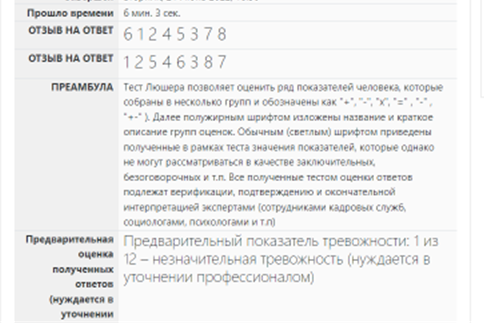
\includegraphics [scale=1.2] {my_folder/images/result35}
	\caption{Результаты теста в версии Moodle 3.5} 
	\label{fig:res35}  
	\end{figure}
\FloatBarrier % заставить рисунки и другие подвижные (float) элементы остановиться
	


	
\section{Тестирование плагинов в Moodle 3.10} \label{ch2:sec-abbr} %название по-русски
Для дальнейшей проверки на компьютере была дополнительно развернута версия 3.10. Установка плагинов прошла без ошибок, однако при попытке создать вопрос в консоли появилась ошибка в файле с Javascript кодом, из-за которой стало невозможно редактировать поля формы. 

На \firef{fig:res310} приведён скриншот результатов теста.
\FloatBarrier % заставить рисунки и другие подвижные (float) элементы остановиться
\begin{figure}[ht] 
	\center
	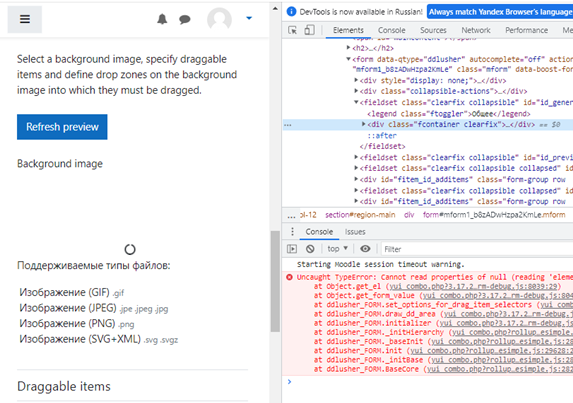
\includegraphics [scale=1] {my_folder/images/result310}
	\caption{Ошибка при попытке создания вопроса в Moodle 3.10} 
	\label{fig:res310}  
\end{figure}
\FloatBarrier % заставить рисунки и другие подвижные (float) элементы остановиться

Плагин поведения протестировать на данном этапе невозможно, так как он зависит от вопроса.
	         	 % Глава 2
\chapter{Реинжиниринг плагинов} \label{ch3}

% не рекомендуется использовать отдельную section <<введение>> после лета 2020 года
%\section{Введение} \label{ch3:intro}

Глава посвящена процессу реинжиниринга плагинов для теста Люшера. Параграф \ref{ch3:sec1} посвящен реинжинирингу плагина вопроса ddlusher. В параграфе \ref{ch3:sec2} описывается процесс анализа и обновления плагина поведения lusherr.
	
\section{Реинжиринг плагина вопроса} \label{ch3:sec1}
%\subsection{Редактирование модуля javascript} % ~ нужен, чтобы избавиться от висячего предлога (союза) в конце строки
На официальном сайте Moodle упоминается, что начиная с Moodle 2.9 осуществляется переход от модулей YUI к модулям AMD, так как команда YUI прекратила новые разработки в библиотеки.\cite{about-yui}

В предыдущей главе было установлено, что ошибка возникает именно в коде модуля YUI, поэтому было принято решение проверить текущий код плагина вопроса перетаскивания изображений на сервере. Как оказалось, в версии 3.10 данный тип вопроса действительно уже использует AMD. 

Далее были проанализированы коды плагина перестаскивания на сервере и плагина вопроса для теста Люшера\cite{psy-test-ddlusher}. В ходе анализа выяснилось, что функции в файлах <<.php>> не изменились, поэтому данные файлы полностью взяты из плагина ddlusher\cite{psy-test-ddlusher}. Однако функции в модулях AMD и YUI уже существенно отличаются. 

Было установлено, что с помощью javascript в ddlusher\cite{psy-test-ddlusher} осуществлялось исчезание карточек после перетаскивания и обновление поля countDrop, которое подсчитывает количество уже выбранных и перенесённых цветов.

За основу был взят код для плагина вопроса с перетаскиванием изображений из папки сервера. В ходе анализа кода модуля в файле question.js была найдена функция dragEnd, которая реагирует на конец перетаскивания. В данную функцию был вставлен код, который скрывает карточку на фоновом изображении и обновляет поле countDrop. Изменения можно найти в строках] \ref{dragEnd}-\ref{dragEnd2} приложения \ref{ap1:sec2}.

Также в файле form.js было скрыто поле, отвечающее за неоднократное перетаскивание элемента на фоновое изображение, и кнопки для добавления новых элементов перетаскивания(строки \ref{hidden}-\ref{hidden2} приложения \ref{ap1:sec1}).

Полный код модуля приведён в приложении \ref{ap1}.

\section{Реинжиниринг плагина поведения} \label{ch3:sec2}

В первую очередь код плагина lusherr\cite{psy-test-lusherr} был проанализирован. Из файла nobutton.js был исключен код, который скрывает кнопку перехода на предыдущий вопрос, так как предотвращение свободного перехода по вопросам можно реализовать в настройках теста.

Также был изменён текст преамбулы, отображающейся в результатах, так как подробная расшифровка теста была исключена автором.

После реинжиниринга плагина вопроса появилась возможность протестировать работу плагина поведения. Переход между вопросами и обработка результатов прошла успешно, в дополнительных доработках данный плагин не нуждается.


           	 % Глава 3
\chapter{Тестирование работы плагинов в тесте} \label{ch4}

% не рекомендуется использовать отдельную section <<введение>> после лета 2020 года
%\section{Введение} \label{ch4:intro}
В главе приведены результаты работы плагинов.
	
\section{Настройка Moodle} \label{ch4:sec1}

Для тестирования работы плагинов в Moodle необходимо выполнить простую установку, загрузив два архива через панель администрирования.

На \firef{fig:zip} приведён скриншот загрузки zip-архива.
\FloatBarrier % заставить рисунки и другие подвижные (float) элементы остановиться
\begin{figure}[ht] 
	\center
	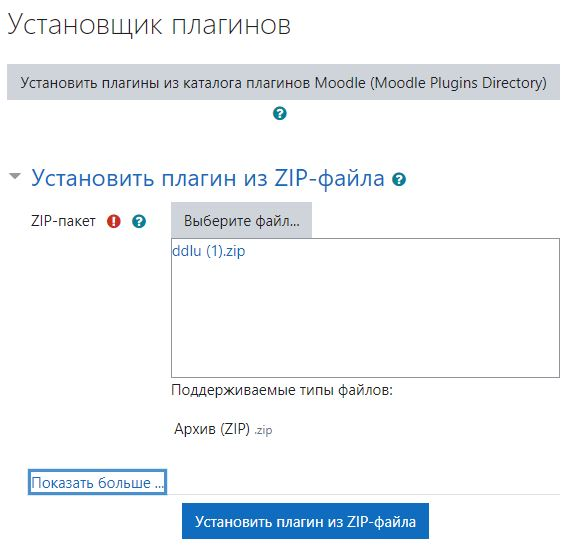
\includegraphics [scale=0.6] {my_folder/images/zip}
	\caption{Загрузка плагинов в Moodle} 
	\label{fig:zip}  
\end{figure}
\FloatBarrier % заставить рисунки и другие подвижные (float) элементы остановиться

Далее нужно создать тест, задать ему имя. Во вкладке <<Расположение>> нужно выбрать метод навигации <<Последовательный>>, в свойствах вопроса настроить режим поведения как пользовательский LusherTest, который мы загрузили ранее. Далее перейдём на вкладку <<Настройки просмотра>>, где уберём все галочки, связанные с баллами и правильными ответами, так система оценивания Moodle не подходит для нашего теста.

На \firef{fig:set1} приведён скриншот с настройками расположения и свойств вопросов.
На \firef{fig:set2} приведены настройки просмотра результатов.
\FloatBarrier % заставить рисунки и другие подвижные (float) элементы остановиться
\begin{figure}[ht] 
	\center
	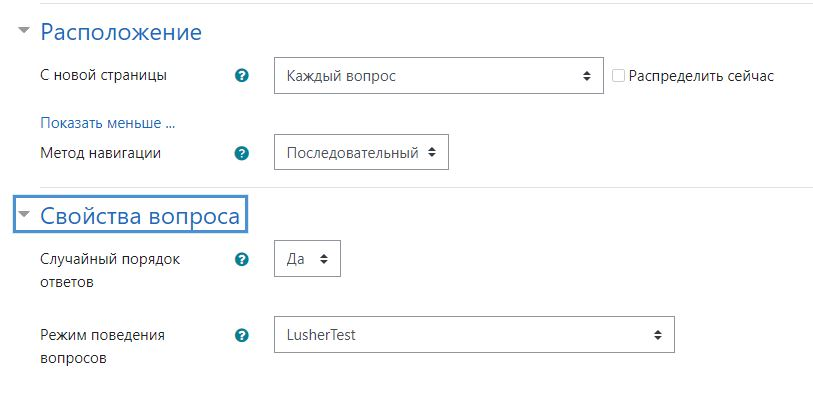
\includegraphics [scale=0.5] {my_folder/images/setting1}
	\caption{Настройки пунктов <<Расположение>> и <<Свойства вопроса>>} 
	\label{fig:set1}  
\end{figure}
\FloatBarrier % заставить рисунки и другие подвижные (float) элементы остановиться
\FloatBarrier % заставить рисунки и другие подвижные (float) элементы остановиться
\begin{figure}[ht] 
	\center
	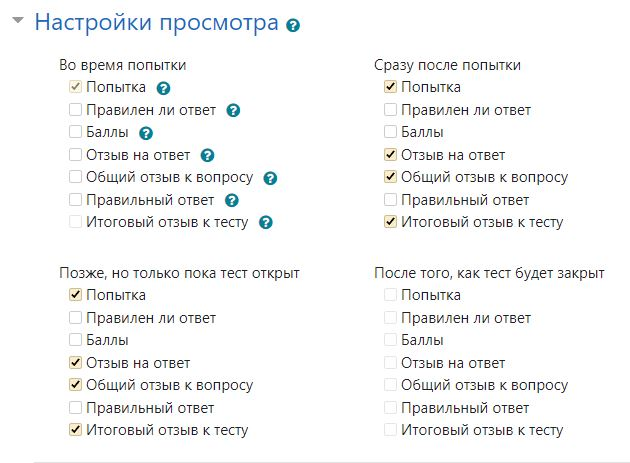
\includegraphics [scale=0.7] {my_folder/images/setting2}
	\caption{Настройки просмотра} 
	\label{fig:set2}  
\end{figure}
\FloatBarrier % заставить рисунки и другие подвижные (float) элементы остановиться
В тесте было создано 2 вопроса загруженного нами типа.

\section{Тестирование работы} \label{ch4:sec2}

После запуска теста на экране появились все карточки и кнопка продолжения, которая не работает, если цвета не перенесены на фоновое изображение. Панель навигации видна, но не работает, как и следовало ожидать. Карточки при перетаскивании исчезали. Исчезновение карточек приведено на \firef{fig:test1}.

\FloatBarrier % заставить рисунки и другие подвижные (float) элементы остановиться
\begin{figure}[ht] 
	\center
	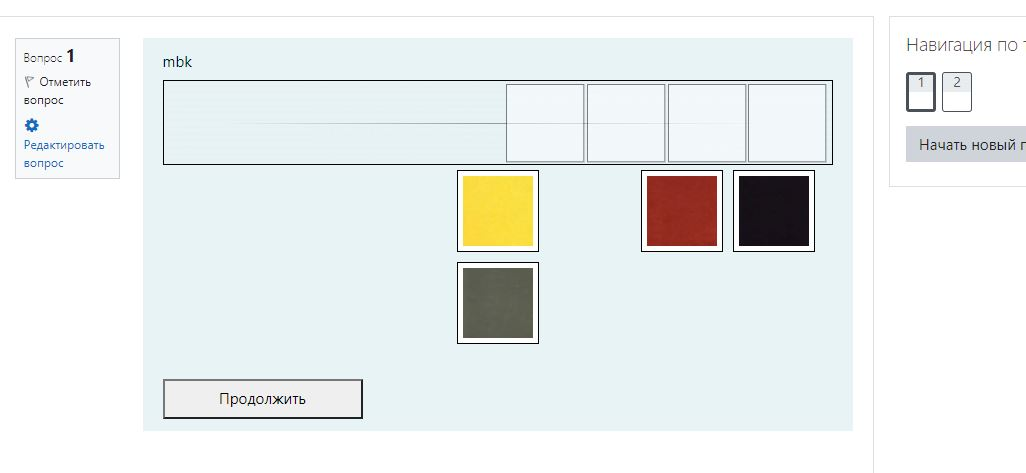
\includegraphics [scale=0.5] {my_folder/images/test1}
	\caption{Исчезновение карточек} 
	\label{fig:test1}  
\end{figure}
\FloatBarrier % заставить рисунки и другие подвижные (float) элементы остановиться

Между вопросами запустился таймер, по истечении времени которого стала доступна кнопка перехода ко второму вопросу. На \firef{fig:time} отображена страница с таймером.
\FloatBarrier % заставить рисунки и другие подвижные (float) элементы остановиться
\begin{figure}[ht] 
	\center
	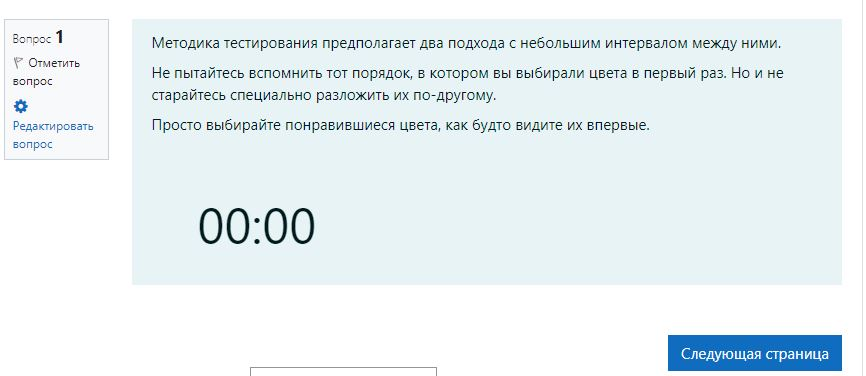
\includegraphics [scale=0.7] {my_folder/images/between}
	\caption{Таймер между вопросами} 
	\label{fig:time}  
\end{figure}
\FloatBarrier % заставить рисунки и другие подвижные (float) элементы остановиться

Тест успешно завершился и показал предварительную оценку тревожности. На \firef{fig:res1} и \firef{fig:res2} можно увидеть страницу отображения результатов теста.
\FloatBarrier % заставить рисунки и другие подвижные (float) элементы остановиться
\begin{figure}[ht] 
	\center
	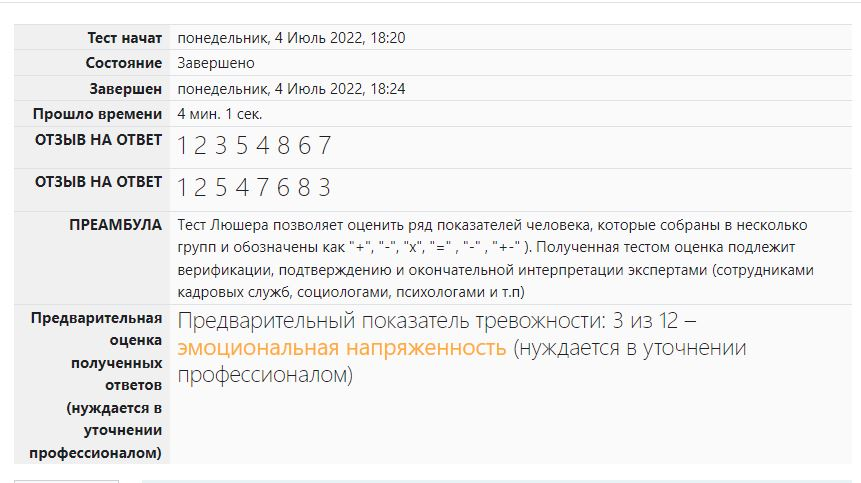
\includegraphics [scale=0.7] {my_folder/images/restest1}
	\caption{Оценка тревожности} 
	\label{fig:res1}  
\end{figure}
\FloatBarrier % заставить рисунки и другие подвижные (float) элементы остановиться

\FloatBarrier % заставить рисунки и другие подвижные (float) элементы остановиться
\begin{figure}[ht] 
	\center
	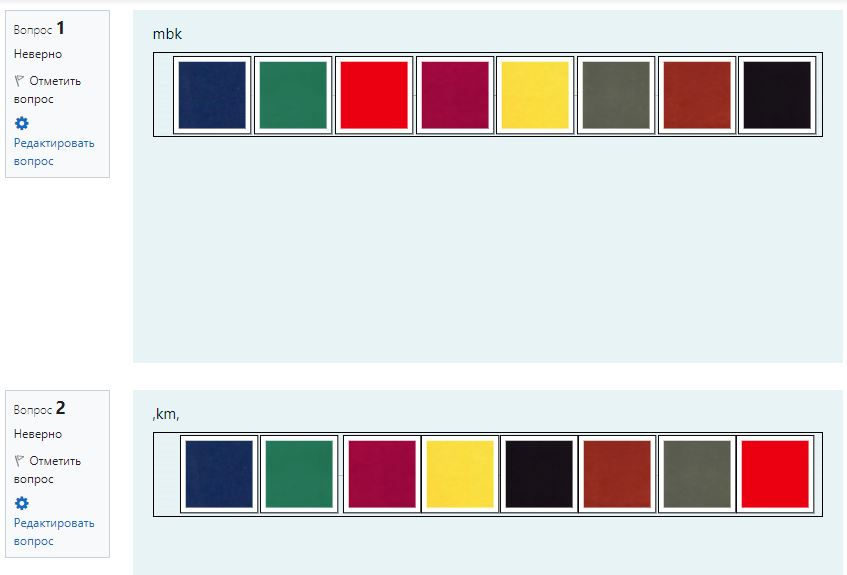
\includegraphics [scale=0.7] {my_folder/images/restest2}
	\caption{Отображение карточек в результатах} 
	\label{fig:res2}  
\end{figure}
\FloatBarrier % заставить рисунки и другие подвижные (float) элементы остановиться
%Пример ссылки на литературу \cite{avtonomova:fya,Peskov2004-ru,Kotelnikov2004-ru,Kotelnikov2004}.

%\FloatBarrier % заставить рисунки и другие подвижные (float) элементы остановиться

%\section{Выводы} \label{ch4:conclusion}

%Текст выводов по главе \thechapter.

%% Вспомогательные команды - Additional commands
%
\newpage % принудительное начало с новой страницы, использовать только в конце раздела
%\clearpage % осуществляется пакетом <<placeins>> в пределах секций
%\newpage\leavevmode\thispagestyle{empty}\newpage % 100 % начало новой страницы           	 % Глава 3
\ContinueChapterEnd % завершить размещение глав <<подряд>>
%% Завершение основной части

\chapter*{Заключение} \label{ch-conclusion}
\addcontentsline{toc}{chapter}{Заключение}	% в оглавление 

В результате пройденной технологической практики была изучена система Moodle, структура плагинов типа вопроса и поведения. Также система Moodle была развёрнута на локальном компьютере.

Существующие плагины для теста Люшера были протестированы в версиях Moodle 3.5 и 3.10. Выявленные ошибки были исправлены путём обновления модуля языка javascript.

Обновлённые плагины были протестированы в Moodle 3.10 на локальном компьютере. Работа теста Люшера прошла успешно, плагины функционируют без ошибок.
        	 % Заключение

%% Наличие следующих перечней не исключает расшифровку сокращения и условного обозначения при первом упоминании в тексте!
%\chapter*{Список сокращений и условных обозначений}             % Заголовок
\addcontentsline{toc}{chapter}{Список сокращений и условных обозначений}  % Добавляем его в оглавление
\noindent
\addtocounter{table}{-1}% Нужно откатить на единицу счетчик номеров таблиц, так как следующая таблица сделана для удобства представления информации по ГОСТ
%\begin{longtabu} to \dimexpr \textwidth-5\tabcolsep {r X}
\begin{longtabu} to \textwidth {r X} % Таблицу не прорисовываем!
% Жирное начертание для математических символов может иметь
% дополнительный смысл, поэтому они приводятся как в тексте
% диссертации
\textbf{DOI} & Digital Object Identifier. \\
\textbf{WoS} & Web of Science. \\
\textbf{ВКР}  & Выпускная квалификационная работа. \\
\textbf{ТГ-объект}  & Текстово-графический объект. \\
%$\begin{rcases}
%a_n\\
%b_n
%\end{rcases}$  & 
%\begin{minipage}{\linewidth}
%Коэффициенты разложения Ми в дальнем поле, соответствующие
%электрическим и магнитным мультиполям.
%\end{minipage}
%\\
%${\boldsymbol{\hat{\mathrm e}}}$ & Единичный вектор. \\
%$E_0$ & Амплитуда падающего поля.\\
%$\begin{rcases}
%a_n\\
%b_n
%\end{rcases}$  & 
%Коэффициенты разложения Ми в дальнем поле соответствующие
%электрическим и магнитным мультиполям ещё раз, но без окружения
%minipage нет вертикального выравнивания по центру.
%\\
%$j$ & Тип функции Бесселя.\\
%$k$ & Волновой вектор падающей волны.\\
%
%$\begin{rcases}
%a_n\\
%b_n
%\end{rcases}$  & 
%\begin{minipage}{\linewidth}
%\vspace{0.7em}
%Коэффициенты разложения Ми в дальнем поле соответствующие
%электрическим и магнитным мультиполям, теперь окружение minipage есть
%и добавленно много текста, так что описание группы условных
%обозначений значительно превысило высоту этой группы... Для отбивки
%пришлось добавить дополнительные отступы.
%\vspace{0.5em}
%\end{minipage}
%\\
%$L$ & Общее число слоёв.\\
%$l$ & Номер слоя внутри стратифицированной сферы.\\
%$\lambda$ & Длина волны электромагнитного излучения
%в вакууме.\\
%$n$ & Порядок мультиполя.\\
%$\begin{rcases}
%{\mathbf{N}}_{e1n}^{(j)}&{\mathbf{N}}_{o1n}^{(j)}\\
%{\mathbf{M}_{o1n}^{(j)}}&{\mathbf{M}_{e1n}^{(j)}}
%\end{rcases}$  & Сферические векторные гармоники.\\
%$\mu$  & Магнитная проницаемость в вакууме.\\
%$r,\theta,\phi$ & Полярные координаты.\\
%$\omega$ & Частота падающей волны.\\
%
%  \textbf{BEM} & Boundary element method, метод граничных элементов.\\
%  \textbf{CST MWS} & Computer Simulation Technology Microwave Studio.

		         % Необязательная рубрика! Список сокращений и условных обозначений

%\chapter*{Словарь терминов}             % Заголовок
\addcontentsline{toc}{chapter}{Словарь терминов}  % Добавляем его в оглавление

\textbf{TeX} --- язык вёрстки текста и издательская система, разработанные Дональдом Кнутом.

\textbf{LaTeX} --- язык вёрстки текста и издательская система, разработанные Лэсли Лампортом как надстройка над TeX.

    		 % Необязательная рубрика! Словарь терминов
% По порядку после Списка сокращений и условных обозначений, если есть.	


\begin{flushleft}
	
\end{flushleft}%%% Не мянять - Do not modify
%%
%%
\clearpage                                  % В том числе гарантирует, что список литературы в оглавлении будет с правильным номером страницы
%\hypersetup{ urlcolor=black }               % Ссылки делаем чёрными
%\providecommand*{\BibDash}{}                % В стилях ugost2008 отключаем использование тире как разделителя 
\urlstyle{rm}                               % ссылки URL обычным шрифтом
\ifdefmacro{\microtypesetup}{\microtypesetup{protrusion=false}}{} % не рекомендуется применять пакет микротипографики к автоматически генерируемому списку литературы
%\newcommand{\fullbibtitle}{Список литературы} % (ГОСТ Р 7.0.11-2011, 4)
%\insertbibliofull  
%\noindent
%\begin{group}
\chapter*{Список использованных источников}	
\label{references}
\addcontentsline{toc}{chapter}{Список использованных источников}	% в оглавление 
\printbibliography[env=SSTfirst]                         % Подключаем Bib-базы
%\ifdefmacro{\microtypesetup}{\microtypesetup{protrusion=true}}{}
%\urlstyle{tt}                               % возвращаем установки шрифта ссылок URL
%\hypersetup{ urlcolor={urlcolor} }          % Восстанавливаем цвет ссылок



%\urlstyle{rm}                               % ссылки URL обычным шрифтом
%\ifdefmacro{\microtypesetup}{\microtypesetup{protrusion=false}}{} % не рекомендуется применять пакет микротипографики к автоматически генерируемому списку литературы
%\insertbibliofull                           % Подключаем Bib-базы
%\ifdefmacro{\microtypesetup}{\microtypesetup{protrusion=true}}{}
%\urlstyle{tt}                               % возвращаем установки шрифта ссылок URL
		     % Список литературы

% Здесь можно поместить список иллюстративного материала

\appendix % не редактировать / keep unmodified


\chapter{Код AMD модуля плагина вопроса}\label{ap1}							% Заголовок
%\addcontentsline{toc}{chapter}{Second call for chapters to participate in the book Machine learning in analysis of biomedical and socio-economic data}	% Добавляем его в оглавление
\lstset{ 
basicstyle=\footnotesize,
breaklines=true,
numbers=left,
stepnumber=5,
escapeinside={(*@}{@*)}
}
\section{form.js} \label{ap1:sec1}
\begin{lstlisting} 
	/*
	* JavaScript to allow dragging options to slots
	* (using mouse down or touch) or tab through slots using keyboard.
	*
	* @module     qtype_ddlu/form
	* @copyright  2018 The Open University
	* @license    http://www.gnu.org/copyleft/gpl.html GNU GPL v3 or later
	*/
	define(['jquery', 'core/dragdrop'], function($, dragDrop) {
		
		"use strict";
		
		/**
		* Singleton object to handle progressive enhancement of the
		* drag-drop onto image question editing form.
		* @type {Object}
		*/
		var dragDropToImageForm = {
			/**
			* @var {Object} maxBgImageSize Properties width and height.
			* @private
			*/
			maxBgImageSize: null,
			
			/**
			* @var {Object} maxDragImageSize with properties width and height.
			* @private
			*/
			maxDragImageSize: null,
			
			/**
			* @property {object} fp for interacting with the file pickers.
			* @private
			*/
			fp: null, // Object containing functions associated with the file picker.
			
			/**
			* Initialise the form javascript features.
			*
			* @method
			*/
			init: function() {
				dragDropToImageForm.fp = dragDropToImageForm.filePickers();
				
				$('#id_previewareaheader').append(
				'<div class="ddarea que ddlu">' +
				'  <div class="droparea">' +
				'    <img class="dropbackground" />' +
				'    <div class="dropzones"></div>' +
				'  </div>' +
				'  <div class="dragitems"></div>' +
				'</div>');
				
				dragDropToImageForm.updateVisibilityOfFilePickers();
				dragDropToImageForm.setOptionsForDragItemSelectors();
				dragDropToImageForm.setupEventHandlers();
				dragDropToImageForm.waitForFilePickerToInitialise();
				//скрываем кнопки добавления(*@\label{hidden}@*)
				var ad = document.getElementsByName("additems");
				ad.item(0).setAttribute("hidden","true");
				var ad = document.getElementsByName("adddropzone");
				ad.item(0).setAttribute("hidden","true");(*@\label{hidden2}@*)
			},
			
			/**
			* Waits for the file-pickers to be sufficiently ready before initialising the preview.
			*/
			waitForFilePickerToInitialise: function() {
				if (dragDropToImageForm.fp.file('bgimage').href === null) {
					// It would be better to use an onload or onchange event rather than this timeout.
					// Unfortunately attempts to do this early are overwritten by filepicker during its loading.
					setTimeout(dragDropToImageForm.waitForFilePickerToInitialise, 1000);
					return;
				}
				M.util.js_pending('dragDropToImageForm');
				
				// From now on, when a new file gets loaded into the filepicker, update the preview.
				// This is not in the setupEventHandlers section as it needs to be delayed until
				// after filepicker's javascript has finished.
				$('form.mform[data-qtype="ddlu"]').on('change', '.filepickerhidden', function() {
					M.util.js_pending('dragDropToImageForm');
					dragDropToImageForm.loadPreviewImage();
				});
				
				dragDropToImageForm.loadPreviewImage();
			},
			
			/**
			* Loads the preview background image.
			*/
			loadPreviewImage: function() {
				$('fieldset#id_previewareaheader .dropbackground')
				.one('load', dragDropToImageForm.afterPreviewImageLoaded)
				.attr('src', dragDropToImageForm.fp.file('bgimage').href);
			},
			
			/**
			* After the background image is loaded, continue setting up the preview.
			*/
			afterPreviewImageLoaded: function() {
				dragDropToImageForm.createDropZones();
				M.util.js_complete('dragDropToImageForm');
			},
			
			/**
			* Create, or recreate all the drop zones.
			*/
			createDropZones: function() {
				var dropZoneHolder = $('.dropzones');
				dropZoneHolder.empty();
				
				var bgimageurl = dragDropToImageForm.fp.file('bgimage').href;
				if (bgimageurl === null) {
					return; // There is not currently a valid preview to update.
				}
				
				var numDrops = dragDropToImageForm.form.getFormValue('nodropzone', []);
				for (var dropNo = 0; dropNo < numDrops; dropNo++) {
					var dragNo = dragDropToImageForm.form.getFormValue('drops',
					[dropNo, 'choice']);
					if (dragNo === '0') {
						continue;
					}
					dragNo = dragNo - 1;
					var group = dragDropToImageForm.form.getFormValue('drags',
					[dragNo, 'draggroup']),
					label = dragDropToImageForm.form.getFormValue('draglabel',
					[dragNo]);
					if ('image' === dragDropToImageForm.form.getFormValue('drags',
					[dragNo, 'dragitemtype'])) {
						var imgUrl = dragDropToImageForm.fp.file('dragitem[' + dragNo + ']').href;
						if (imgUrl === null) {
							continue;
						}
						// Althoug these are previews of drops, we also add the class name 'drag',
						dropZoneHolder.append('<img class="droppreview group' + group + ' drop' + dropNo +
						'" src="' + imgUrl + '" alt="' + label + '" data-drop-no="' + dropNo + '">');
						
					} else if (label !== '') {
						dropZoneHolder.append('<div class="droppreview group' + group + ' drop' + dropNo +
						'"  data-drop-no="' + dropNo + '">' + label + '</div>');
					}
				}
				
				dragDropToImageForm.waitForAllDropImagesToBeLoaded();
			},
			
			/**
			* This polls until all the drop-zone images have loaded, and then calls updateDropZones().
			*/
			waitForAllDropImagesToBeLoaded: function() {
				var notYetLoadedImages = $('.dropzones img').not(function(i, imgNode) {
					return dragDropToImageForm.imageIsLoaded(imgNode);
				});
				
				if (notYetLoadedImages.length > 0) {
					setTimeout(function() {
						dragDropToImageForm.waitForAllDropImagesToBeLoaded();
					}, 100);
					return;
				}
				
				dragDropToImageForm.updateDropZones();
			},
			
			/**
			* Check if an image has loaded without errors.
			*
			* @param {HTMLImageElement} imgElement an image.
			* @returns {boolean} true if this image has loaded without errors.
			*/
			imageIsLoaded: function(imgElement) {
				return imgElement.complete && imgElement.naturalHeight !== 0;
			},
			
			/**
			* Set the size and position of all the drop zones.
			*/
			updateDropZones: function() {
				var bgimageurl = dragDropToImageForm.fp.file('bgimage').href;
				if (bgimageurl === null) {
					return; // There is not currently a valid preview to update.
				}
				
				var dropBackgroundPosition = $('fieldset#id_previewareaheader .dropbackground').offset(),
				numDrops = dragDropToImageForm.form.getFormValue('nodropzone', []);
				
				// Move each drop to the right position and update the text.
				for (var dropNo = 0; dropNo < numDrops; dropNo++) {
					var drop = $('.dropzones .drop' + dropNo);
					if (drop.length === 0) {
						continue;
					}
					var dragNo = dragDropToImageForm.form.getFormValue('drops',
					[dropNo, 'choice']) - 1;
					
					drop.offset({
						left: dropBackgroundPosition.left +
						parseInt(dragDropToImageForm.form.getFormValue('drops',
						[dropNo, 'xleft'])),
						top: dropBackgroundPosition.top +
						parseInt(dragDropToImageForm.form.getFormValue('drops',
						[dropNo, 'ytop']))
					});
					
					var label = dragDropToImageForm.form.getFormValue('draglabel', [dragNo]);
					if (drop.is('img')) {
						drop.attr('alt', label);
					} else {
						drop.html(label);
					}
				}
				
				// Resize them to the same size.
				$('.dropzones .droppreview').css('padding', '0');
				var numGroups = $('.draggroup select').first().find('option').length;
				for (var group = 1; group <= numGroups; group++) {
					dragDropToImageForm.resizeAllDragsAndDropsInGroup(group);
				}
			},
			
			/**
			* In a given group, set all the drags and drops to be the same size.
			*
			* @param {int} group the group number.
			*/
			resizeAllDragsAndDropsInGroup: function(group) {
				var drops = $('.dropzones .droppreview.group' + group),
				maxWidth = 0,
				maxHeight = 0;
				
				// Find the maximum size of any drag in this groups.
				drops.each(function(i, drop) {
					maxWidth = Math.max(maxWidth, Math.ceil(drop.offsetWidth));
					maxHeight = Math.max(maxHeight, Math.ceil(drop.offsetHeight));
				});
				
				// The size we will want to set is a bit bigger than this.
				maxWidth += 10;
				maxHeight += 10;
				
				// Set each drag home to that size.
				drops.each(function(i, drop) {
					var left = Math.round((maxWidth - drop.offsetWidth) / 2),
					top = Math.floor((maxHeight - drop.offsetHeight) / 2);
					// Set top and left padding so the item is centred.
					$(drop).css({
						'padding-left': left + 'px',
						'padding-right': (maxWidth - drop.offsetWidth - left) + 'px',
						'padding-top': top + 'px',
						'padding-bottom': (maxHeight - drop.offsetHeight - top) + 'px'
					});
				});
			},
			
			/**
			* Events linked to form actions.
			*/
			setupEventHandlers: function() {
				// Changes to settings in the draggable items section.
				$('fieldset#id_draggableitemheader')
				.on('change input', 'input, select', function(e) {
					var input = $(e.target).closest('select, input');
					if (input.hasClass('dragitemtype')) {
						dragDropToImageForm.updateVisibilityOfFilePickers();
					}
					
					dragDropToImageForm.setOptionsForDragItemSelectors();
					
					if (input.is('.dragitemtype, .draggroup')) {
						dragDropToImageForm.createDropZones();
					} else if (input.is('.draglabel')) {
						dragDropToImageForm.updateDropZones();
					}
				});
				
				// Changes to Drop zones section: left, top and drag item.
				$('fieldset#id_dropzoneheader').on('change input', 'input, select', function(e) {
					var input = $(e.target).closest('select, input');
					if (input.is('select')) {
						dragDropToImageForm.createDropZones();
					} else {
						dragDropToImageForm.updateDropZones();
					}
				});
				
				// Moving drop zones in the preview.
				$('fieldset#id_previewareaheader').on('mousedown touchstart', '.droppreview', function(e) {
					dragDropToImageForm.dragStart(e);
				});
				
				$(window).on('resize', function() {
					dragDropToImageForm.updateDropZones();
				});
			},
			
			/**
			* Update all the drag item filepickers, so they are only shown for
			*/
			updateVisibilityOfFilePickers: function() {
				var numDrags = dragDropToImageForm.form.getFormValue('noitems', []);
				for (var dragNo = 0; dragNo < numDrags; dragNo++) {
					var picker = $('input#id_dragitem_' + dragNo).closest('.fitem_ffilepicker');
					if ('image' === dragDropToImageForm.form.getFormValue('drags',
					[dragNo, 'dragitemtype'])) {
						picker.show();
					} else {
						picker.hide();
					}
				}
			},
			
			
			setOptionsForDragItemSelectors: function() {
				var dragItemOptions = {'0': ''},
				numDrags = dragDropToImageForm.form.getFormValue('noitems', []),
				numDrops = dragDropToImageForm.form.getFormValue('nodropzone', []);
				
				// Work out the list of options.
				for (var dragNo = 0; dragNo < numDrags; dragNo++) {
					var label = dragDropToImageForm.form.getFormValue('draglabel', [dragNo]);
					var file =
					dragDropToImageForm.fp.file(dragDropToImageForm.form.toNameWithIndex('dragitem',
					[dragNo]));
					if ('image' === dragDropToImageForm.form.getFormValue('drags',
					[dragNo, 'dragitemtype']) && file.name !== null) {
						dragItemOptions[dragNo + 1] = (dragNo + 1) + '. ' + label + ' (' + file.name + ')';
					} else if (label !== '') {
						dragItemOptions[dragNo + 1] = (dragNo + 1) + '. ' + label;
					}
				}
				
				// Initialise each select.
				for (var dropNo = 0; dropNo < numDrops; dropNo++) {
					var selector = $('#id_drops_' + dropNo + '_choice');
					
					var selectedvalue = selector.val();
					selector.find('option').remove();
					for (var value in dragItemOptions) {
						if (!dragItemOptions.hasOwnProperty(value)) {
							continue;
						}
						selector.append('<option value="' + value + '">'
						+ dragItemOptions[value] + '</option>');
						var optionnode = selector.find('option[value="' + value + '"]');
						if (parseInt(value) === parseInt(selectedvalue)) {
							optionnode.attr('selected', true);
						} else if (dragDropToImageForm.isItemUsed(parseInt(value))) {
							optionnode.attr('disabled', true);
						}
					}
				}
			},
			
			/**
			* Checks if the specified drag option is already used somewhere.
			*
			* @param {Number} value of the drag item to check
			* @return {Boolean} true if item is allocated to dropzone
			*/
			isItemUsed: function(value) {
				if (value === 0) {
					return false; // None option can always be selected.
				}
				
				return $('fieldset#id_dropzoneheader select').filter(function(i, selectNode) {
					return parseInt($(selectNode).val()) === value;
				}).length !== 0;
			},
			
			/**
			* Handles when a dropzone in dragged in the preview.
			* @param {Object} e Event object
			*/
			dragStart: function(e) {
				var drop = $(e.target).closest('.droppreview');
				
				var info = dragDrop.prepare(e);
				if (!info.start) {
					return;
				}
				
				dragDrop.start(e, drop, function(x, y, drop) {
					dragDropToImageForm.dragMove(drop);
				}, function() {
					dragDropToImageForm.dragEnd();
				});
			},
			
			/**
			* Handles update while a drop is being dragged.
			*
			* @param {jQuery} drop the drop preview being moved.
			*/
			dragMove: function(drop) {
				var backgroundImage = $('fieldset#id_previewareaheader .dropbackground'),
				backgroundPosition = backgroundImage.offset(),
				dropNo = drop.data('dropNo'),
				dropPosition = drop.offset(),
				left = Math.round(dropPosition.left - backgroundPosition.left),
				top = Math.round(dropPosition.top - backgroundPosition.top);
				
				// Constrain coordinates to be inside the background.
				left = Math.round(Math.max(0, Math.min(left, backgroundImage.outerWidth()
				- drop.outerWidth())));
				top = Math.round(Math.max(0, Math.min(top, backgroundImage.outerHeight()
				- drop.outerHeight())));
				
				// Update the form.
				dragDropToImageForm.form.setFormValue('drops', [dropNo, 'xleft'], left);
				dragDropToImageForm.form.setFormValue('drops', [dropNo, 'ytop'], top);
			},
			
			/**
			* Handles when the drag ends.
			*/
			dragEnd: function() {
				// Redraw, in case the position was constrained.
				dragDropToImageForm.updateDropZones();
			},
			
			/**
			* Low level operations on form.
			*/
			form: {
				toNameWithIndex: function(name, indexes) {
					var indexString = name;
					for (var i = 0; i < indexes.length; i++) {
						indexString = indexString + '[' + indexes[i] + ']';
					}
					return indexString;
				},
				
				getEl: function(name, indexes) {
					var form = $('form.mform[data-qtype="ddlu"]')[0];
					return form.elements[this.toNameWithIndex(name, indexes)];
				},
				
				/**
				* Helper to get the value of a form elements with name like "drops[0][xleft]".
				*
				* @param {String} name the base name, e.g. 'drops'.
				* @param {String[]} indexes the indexes, e.g. ['0', 'xleft'].
				* @return {String} the value of that field.
				*/
				getFormValue: function(name, indexes) {
					var el = this.getEl(name, indexes);
					if (!el.type) {
						el = el[el.length - 1];
					}
					if (el.type === 'checkbox') {
						return el.checked;
					} else {
						return el.value;
					}
				},
				
				/**
				* Helper to get the value of a form elements with name like "drops[0][xleft]".
				*
				* @param {String} name the base name, e.g. 'drops'.
				* @param {String[]} indexes the indexes, e.g. ['0', 'xleft'].
				* @param {String|Number} value the value to set.
				*/
				setFormValue: function(name, indexes, value) {
					var el = this.getEl(name, indexes);
					if (el.type === 'checkbox') {
						el.checked = value;
					} else {
						el.value = value;
					}
				}
			},
			
			/**
			* Utility to get the file name and url from the filepicker.
			* @returns {Object} object containing functions {file, name}
			*/
			filePickers: function() {
				var draftItemIdsToName;
				var nameToParentNode;
				
				if (draftItemIdsToName === undefined) {
					draftItemIdsToName = {};
					nameToParentNode = {};
					var fp = $('form.mform[data-qtype="ddlu"] input.filepickerhidden');
					fp.each(function(index, filepicker) {
						draftItemIdsToName[filepicker.value] = filepicker.name;
						nameToParentNode[filepicker.name] = filepicker.parentNode;
					});
				}
				
				return {
					file: function(name) {
						var parentNode = $(nameToParentNode[name]);
						var fileAnchor = parentNode.find('div.filepicker-filelist a');
						if (fileAnchor.length) {
							return {href: fileAnchor.get(0).href, name: fileAnchor.get(0).innerHTML};
						} else {
							return {href: null, name: null};
						}
					},
					
					name: function(draftitemid) {
						return draftItemIdsToName[draftitemid];
					}
				};
			}
		};
		
		return {
			init: dragDropToImageForm.init
		};
	});
	
\end{lstlisting}

\section{question.js} \label{ap1:sec2}
\begin{lstlisting} 
	/*
	* JavaScript to allow dragging options to slots (using mouse down or touch) or tab through slots using keyboard.
	*
	* @module     qtype_ddlu/question
	* @copyright  2018 The Open University
	* @license    http://www.gnu.org/copyleft/gpl.html GNU GPL v3 or later
	*/
	define(['jquery', 'core/dragdrop', 'core/key_codes'], function($, dragDrop, keys) {
		
		"use strict";
		
		/**
		* Initialise one drag-drop onto image question.
		*
		* @param {String} containerId id of the outer div for this question.
		* @param {boolean} readOnly whether the question is being displayed read-only.
		* @param {Array} places Information about the drop places.
		* @constructor
		*/
		function DragDropOntoImageQuestion(containerId, readOnly, places) {
			this.containerId = containerId;
			M.util.js_pending('qtype_ddlu-init-' + this.containerId);
			this.places = places;
			this.allImagesLoaded = false;
			this.imageLoadingTimeoutId = null;
			this.isPrinting = false;
			if (readOnly) {
				this.getRoot().addClass('qtype_ddlu-readonly');
			}
			
			var thisQ = this;
			this.getNotYetLoadedImages().one('load', function() {
				thisQ.waitForAllImagesToBeLoaded();
			});
			this.waitForAllImagesToBeLoaded();
		}
		
		/**
		* Waits until all images are loaded before calling setupQuestion().
		*
		* This function is called from the onLoad of each image, and also polls with
		* a time-out, because image on-loads are allegedly unreliable.
		*/
		DragDropOntoImageQuestion.prototype.waitForAllImagesToBeLoaded = function() {
			var thisQ = this;
			
			// This method may get called multiple times (via image on-loads or timeouts.
			// If we are already done, don't do it again.
			if (this.allImagesLoaded) {
				return;
			}
			
			// Clear any current timeout, if set.
			if (this.imageLoadingTimeoutId !== null) {
				clearTimeout(this.imageLoadingTimeoutId);
			}
			
			// If we have not yet loaded all images, set a timeout to
			// call ourselves again, since apparently images on-load
			// events are flakey.
			if (this.getNotYetLoadedImages().length > 0) {
				this.imageLoadingTimeoutId = setTimeout(function() {
					thisQ.waitForAllImagesToBeLoaded();
				}, 100);
				return;
			}
			
			// We now have all images. Carry on, but only after giving the layout a chance to settle down.
			this.allImagesLoaded = true;
			thisQ.setupQuestion();
		};
		
		/**
		* Get any of the images in the drag-drop area that are not yet fully loaded.
		*
		* @returns {jQuery} those images.
		*/
		DragDropOntoImageQuestion.prototype.getNotYetLoadedImages = function() {
			var thisQ = this;
			return this.getRoot().find('.ddarea img').not(function(i, imgNode) {
				return thisQ.imageIsLoaded(imgNode);
			});
		};
		
		/**
		* Check if an image has loaded without errors.
		*
		* @param {HTMLImageElement} imgElement an image.
		* @returns {boolean} true if this image has loaded without errors.
		*/
		DragDropOntoImageQuestion.prototype.imageIsLoaded = function(imgElement) {
			return imgElement.complete && imgElement.naturalHeight !== 0;
		};
		
		/**
		* Set up the question, once all images have been loaded.
		*/
		DragDropOntoImageQuestion.prototype.setupQuestion = function() {
			this.resizeAllDragsAndDrops();
			this.cloneDrags();
			this.positionDragsAndDrops();
			M.util.js_complete('qtype_ddlu-init-' + this.containerId);
		};
		
		/**
		* In each group, resize all the items to be the same size.
		*/
		DragDropOntoImageQuestion.prototype.resizeAllDragsAndDrops = function() {
			var thisQ = this;
			this.getRoot().find('.draghomes > div').each(function(i, node) {
				thisQ.resizeAllDragsAndDropsInGroup(
				thisQ.getClassnameNumericSuffix($(node), 'dragitemgroup'));
			});
		};
		
		/**
		* In a given group, set all the drags and drops to be the same size.
		*
		* @param {int} group the group number.
		*/
		DragDropOntoImageQuestion.prototype.resizeAllDragsAndDropsInGroup = function(group) {
			var root = this.getRoot(),
			dragHomes = root.find('.dragitemgroup' + group + ' .draghome'),
			maxWidth = 0,
			maxHeight = 0;
			
			// Find the maximum size of any drag in this groups.
			dragHomes.each(function(i, drag) {
				maxWidth = Math.max(maxWidth, Math.ceil(drag.offsetWidth));
				maxHeight = Math.max(maxHeight, Math.ceil(drag.offsetHeight));
			});
			
			// The size we will want to set is a bit bigger than this.
			maxWidth += 10;
			maxHeight += 10;
			
			// Set each drag home to that size.
			dragHomes.each(function(i, drag) {
				var left = Math.round((maxWidth - drag.offsetWidth) / 2),
				top = Math.floor((maxHeight - drag.offsetHeight) / 2);
				// Set top and left padding so the item is centred.
				$(drag).css({
					'padding-left': left + 'px',
					'padding-right': (maxWidth - drag.offsetWidth - left) + 'px',
					'padding-top': top + 'px',
					'padding-bottom': (maxHeight - drag.offsetHeight - top) + 'px'
				});
			});
			
			// Create the drops and make them the right size.
			for (var i in this.places) {
				if (!this.places.hasOwnProperty((i))) {
					continue;
				}
				var place = this.places[i],
				label = place.text;
				if (parseInt(place.group) !== group) {
					continue;
				}
				if (label === '') {
					label = M.util.get_string('blank', 'qtype_ddlu');
				}
				root.find('.dropzones').append('<div class="dropzone active group' + place.group +
				' place' + i + '" tabindex="0">' +
				'<span class="accesshide">' + label + '</span>&nbsp;</div>');
				root.find('.dropzone.place' + i).width(maxWidth - 2).height(maxHeight - 2);
			}
		};
		
		/**
		* Invisible 'drag homes' are output by the renderer. These have the same properties
		* as the drag items but are invisible. We clone these invisible elements to make the
		* actual drag items.
		*/
		DragDropOntoImageQuestion.prototype.cloneDrags = function() {
			var thisQ = this;
			thisQ.getRoot().find('.draghome').each(function(index, dragHome) {
				var drag = $(dragHome);
				var placeHolder = drag.clone();
				placeHolder.removeClass();
				placeHolder.addClass('draghome choice' +
				thisQ.getChoice(drag) + ' group' +
				thisQ.getGroup(drag) + ' dragplaceholder');
				drag.before(placeHolder);
			});
		};
		
		
		/**
		* Update the position of drags.
		*/
		DragDropOntoImageQuestion.prototype.positionDragsAndDrops = function() {
			var thisQ = this,
			root = this.getRoot(),
			bgRatio = this.bgRatio();
			
			// Move the drops into position.
			root.find('.ddarea .dropzone').each(function(i, dropNode) {
				var drop = $(dropNode),
				place = thisQ.places[thisQ.getPlace(drop)];
				// The xy values come from PHP as strings, so we need parseInt to stop JS doing string concatenation.
				drop.css('left', parseInt(place.xy[0]) * bgRatio)
				.css('top', parseInt(place.xy[1]) * bgRatio);
				drop.data('originX', parseInt(place.xy[0]))
				.data('originY', parseInt(place.xy[1]));
				thisQ.handleElementScale(drop, 'left top');
			});
			
			// First move all items back home.
			root.find('.draghome').not('.dragplaceholder').each(function(i, dragNode) {
				var drag = $(dragNode),
				currentPlace = thisQ.getClassnameNumericSuffix(drag, 'inplace');
				drag.addClass('unplaced')
				.removeClass('placed');
				drag.removeAttr('tabindex');
				if (currentPlace !== null) {
					drag.removeClass('inplace' + currentPlace);
				}
			});
			
			// Then place the ones that should be placed.
			root.find('input.placeinput').each(function(i, inputNode) {
				var input = $(inputNode),
				choice = input.val();
				if (choice.length === 0 || (choice.length > 0 && choice === '0')) {
					// No item in this place.
					return;
				}
				
				var place = thisQ.getPlace(input);
				// Get the unplaced drag.
				var unplacedDrag = thisQ.getUnplacedChoice(thisQ.getGroup(input), choice);
				// Get the clone of the drag.
				var hiddenDrag = thisQ.getDragClone(unplacedDrag);
				if (hiddenDrag.length) {
					hiddenDrag.addClass('active');
					
				}
				
				// Send the drag to drop.
				var drop = root.find('.dropzone.place' + place);
				thisQ.sendDragToDrop(unplacedDrag, drop);
				var page = document.location.href;
				if(!page.includes('review')){
					var an = unplacedDrag.attr('class');
					document.getElementsByClassName(an)[0].setAttribute('hidden',true);
				}
			});
		};
		
		/**
		* Handles the start of dragging an item.
		*
		* @param {Event} e the touch start or mouse down event.
		*/
		DragDropOntoImageQuestion.prototype.handleDragStart = function(e) {
			var thisQ = this,
			drag = $(e.target).closest('.draghome'),
			currentIndex = this.calculateZIndex(),
			newIndex = currentIndex + 2;
			
			var info = dragDrop.prepare(e);
			if (!info.start || drag.hasClass('beingdragged')) {
				return;
			}
			
			drag.addClass('beingdragged').css('transform', '').css('z-index', newIndex);
			var currentPlace = this.getClassnameNumericSuffix(drag, 'inplace');
			if (currentPlace !== null) {
				this.setInputValue(currentPlace, 0);
				drag.removeClass('inplace' + currentPlace);
				var hiddenDrop = thisQ.getDrop(drag, currentPlace);
				if (hiddenDrop.length) {
					hiddenDrop.addClass('active');
					drag.offset(hiddenDrop.offset());
				}
			} else {
				var hiddenDrag = thisQ.getDragClone(drag);
				if (hiddenDrag.length) {
					hiddenDrag.addClass('active');
					drag.offset(hiddenDrag.offset());
				}
			}
			
			dragDrop.start(e, drag, function(x, y, drag) {
				thisQ.dragMove(x, y, drag);
			}, function(x, y, drag) {
				thisQ.dragEnd(x, y, drag);
			});
		};
		
		/**
		* Called whenever the currently dragged items moves.
		*
		* @param {Number} pageX the x position.
		* @param {Number} pageY the y position.
		* @param {jQuery} drag the item being moved.
		*/
		DragDropOntoImageQuestion.prototype.dragMove = function(pageX, pageY, drag) {
			var thisQ = this,
			highlighted = false;
			this.getRoot().find('.dropzone.group' + this.getGroup(drag)).each(function(i, dropNode) {
				var drop = $(dropNode);
				if (thisQ.isPointInDrop(pageX, pageY, drop) && !highlighted) {
					highlighted = true;
					drop.addClass('valid-drag-over-drop');
				} else {
					drop.removeClass('valid-drag-over-drop');
				}
			});
			this.getRoot().find('.draghome.placed.group' + this.getGroup(drag)).not('.beingdragged').each(function(i, dropNode) {
				var drop = $(dropNode);
				if (thisQ.isPointInDrop(pageX, pageY, drop) && !highlighted && !thisQ.isDragSameAsDrop(drag, drop)) {
					highlighted = true;
					drop.addClass('valid-drag-over-drop');
				} else {
					drop.removeClass('valid-drag-over-drop');
				}
			});
		};
		
		/**
		* Called when user drops a drag item.
		*
		* @param {Number} pageX the x position.
		* @param {Number} pageY the y position.
		* @param {jQuery} drag the item being moved.
		*/
		DragDropOntoImageQuestion.prototype.dragEnd = function(pageX, pageY, drag)  {
			var thisQ = this,
			root = this.getRoot(),
			placed = false;
			
			// Looking for drag that was dropped on a dropzone.
			root.find('.dropzone.group' + this.getGroup(drag)).each(function(i, dropNode) {
				var drop = $(dropNode);
				if (!thisQ.isPointInDrop(pageX, pageY, drop)) {
					// Not this drop.
					return true;
				}
				
				// Now put this drag into the drop.
				drop.removeClass('valid-drag-over-drop');
				thisQ.sendDragToDrop(drag, drop);
				placed = true;
				//СОКРЫТИЕ КАРТОЧКИ И ОБНОВЛЕНИЕ КОЛИЧЕСТВА(*@\label{dragEnd}@*)
				var an = drag.attr('class');
				document.getElementsByClassName(an)[0].setAttribute('hidden',true);
				var num = document.getElementById("countDrop").innerHTML;
				document.getElementById("countDrop").innerHTML =  parseInt(num) + parseInt(1);(*@\label{dragEnd2}@*)
				return false; // Stop the each() here.
			});
			
			if (!placed) {
				// Looking for that was dropped on a placed drag.
				root.find('.draghome.placed.group' + this.getGroup(drag)).not('.beingdragged').each(function(i, placedNode) {
					var placedDrag = $(placedNode);
					if (!thisQ.isPointInDrop(pageX, pageY, placedDrag) || thisQ.isDragSameAsDrop(drag, placedDrag)) {
						// Not this placed drag.
						return true;
					}
					
					// Now put this drag into the drop.
					placedDrag.removeClass('valid-drag-over-drop');
					var currentPlace = thisQ.getClassnameNumericSuffix(placedDrag, 'inplace');
					var drop = thisQ.getDrop(drag, currentPlace);
					thisQ.sendDragToDrop(drag, drop);
					placed = true;
					return false; // Stop the each() here.
				});
			}
			
			if (!placed) {
				this.sendDragHome(drag);
			}
		};
		
		/**
		* Animate a drag item into a given place (or back home).
		*
		* @param {jQuery|null} drag the item to place. If null, clear the place.
		* @param {jQuery} drop the place to put it.
		*/
		DragDropOntoImageQuestion.prototype.sendDragToDrop = function(drag, drop) {
			// Is there already a drag in this drop? if so, evict it.
			var oldDrag = this.getCurrentDragInPlace(this.getPlace(drop));
			if (oldDrag.length !== 0) {
				oldDrag.addClass('beingdragged');
				oldDrag.offset(oldDrag.offset());
				var currentPlace = this.getClassnameNumericSuffix(oldDrag, 'inplace');
				var hiddenDrop = this.getDrop(oldDrag, currentPlace);
				hiddenDrop.addClass('active');
				this.sendDragHome(oldDrag);
			}
			
			if (drag.length === 0) {
				this.setInputValue(this.getPlace(drop), 0);
				if (drop.data('isfocus')) {
					drop.focus();
				}
			} else {
				this.setInputValue(this.getPlace(drop), this.getChoice(drag));
				drag.removeClass('unplaced')
				.addClass('placed inplace' + this.getPlace(drop));
				
				drag.attr('tabindex', 0);
				this.animateTo(drag, drop);
				
			}
		};
		
		/**
		* Animate a drag back to its home.
		*
		* @param {jQuery} drag the item being moved.
		*/
		DragDropOntoImageQuestion.prototype.sendDragHome = function(drag) {
			var currentPlace = this.getClassnameNumericSuffix(drag, 'inplace');
			if (currentPlace !== null) {
				drag.removeClass('inplace' + currentPlace);
			}
			drag.data('unplaced', true);
			
			this.animateTo(drag, this.getDragHome(this.getGroup(drag), this.getChoice(drag)));
		};
		
		/**
		* Handles keyboard events on drops.
		*
		* Drops are focusable. Once focused, right/down/space switches to the next choice, and
		* left/up switches to the previous. Escape clear.
		*
		* @param {KeyboardEvent} e
		*/
		DragDropOntoImageQuestion.prototype.handleKeyPress = function(e) {
			var drop = $(e.target).closest('.dropzone');
			if (drop.length === 0) {
				var placedDrag = $(e.target);
				var currentPlace = this.getClassnameNumericSuffix(placedDrag, 'inplace');
				if (currentPlace !== null) {
					drop = this.getDrop(placedDrag, currentPlace);
				}
			}
			var currentDrag = this.getCurrentDragInPlace(this.getPlace(drop)),
			nextDrag = $();
			
			switch (e.keyCode) {
				case keys.space:
				case keys.arrowRight:
				case keys.arrowDown:
				nextDrag = this.getNextDrag(this.getGroup(drop), currentDrag);
				break;
				
				case keys.arrowLeft:
				case keys.arrowUp:
				nextDrag = this.getPreviousDrag(this.getGroup(drop), currentDrag);
				break;
				
				case keys.escape:
				questionManager.isKeyboardNavigation = false;
				break;
				
				default:
				questionManager.isKeyboardNavigation = false;
				return; // To avoid the preventDefault below.
			}
			
			if (nextDrag.length) {
				nextDrag.data('isfocus', true);
				nextDrag.addClass('beingdragged');
				var hiddenDrag = this.getDragClone(nextDrag);
				if (hiddenDrag.length) {
					hiddenDrag.addClass('active');
					nextDrag.offset(hiddenDrag.offset());
				}
			} else {
				drop.data('isfocus', true);
			}
			
			e.preventDefault();
			this.sendDragToDrop(nextDrag, drop);
		};
		
		/**
		* Choose the next drag in a group.
		*
		* @param {int} group which group.
		* @param {jQuery} drag current choice (empty jQuery if there isn't one).
		* @return {jQuery} the next drag in that group, or null if there wasn't one.
		*/
		DragDropOntoImageQuestion.prototype.getNextDrag = function(group, drag) {
			var choice,
			numChoices = this.noOfChoicesInGroup(group);
			
			if (drag.length === 0) {
				choice = 1; // Was empty, so we want to select the first choice.
			} else {
				choice = this.getChoice(drag) + 1;
			}
			
			var next = this.getUnplacedChoice(group, choice);
			while (next.length === 0 && choice < numChoices) {
				choice++;
				next = this.getUnplacedChoice(group, choice);
			}
			
			return next;
		};
		
		/**
		* Choose the previous drag in a group.
		*
		* @param {int} group which group.
		* @param {jQuery} drag current choice (empty jQuery if there isn't one).
		* @return {jQuery} the next drag in that group, or null if there wasn't one.
		*/
		DragDropOntoImageQuestion.prototype.getPreviousDrag = function(group, drag) {
			var choice;
			
			if (drag.length === 0) {
				choice = this.noOfChoicesInGroup(group);
			} else {
				choice = this.getChoice(drag) - 1;
			}
			
			var previous = this.getUnplacedChoice(group, choice);
			while (previous.length === 0 && choice > 1) {
				choice--;
				previous = this.getUnplacedChoice(group, choice);
			}
			
			// Does this choice exist?
			return previous;
		};
		
		/**
		* Animate an object to the given destination.
		*
		* @param {jQuery} drag the element to be animated.
		* @param {jQuery} target element marking the place to move it to.
		*/
		DragDropOntoImageQuestion.prototype.animateTo = function(drag, target) {
			var currentPos = drag.offset(),
			targetPos = target.offset(),
			thisQ = this;
			
			M.util.js_pending('qtype_ddlu-animate-' + thisQ.containerId);
			// Animate works in terms of CSS position, whereas locating an object
			// on the page works best with jQuery offset() function. So, to get
			// the right target position, we work out the required change in
			// offset() and then add that to the current CSS position.
			drag.animate(
			{
				left: parseInt(drag.css('left')) + targetPos.left - currentPos.left,
				top: parseInt(drag.css('top')) + targetPos.top - currentPos.top
			},
			{
				duration: 'fast',
				done: function() {
					$('body').trigger('qtype_ddlu-dragmoved', [drag, target, thisQ]);
					M.util.js_complete('qtype_ddlu-animate-' + thisQ.containerId);
				}
			}
			);
		};
		
		/**
		* Detect if a point is inside a given DOM node.
		*
		* @param {Number} pageX the x position.
		* @param {Number} pageY the y position.
		* @param {jQuery} drop the node to check (typically a drop).
		* @return {boolean} whether the point is inside the node.
		*/
		DragDropOntoImageQuestion.prototype.isPointInDrop = function(pageX, pageY, drop) {
			var position = drop.offset();
			if (drop.hasClass('draghome')) {
				return pageX >= position.left && pageX < position.left + drop.outerWidth()
				&& pageY >= position.top && pageY < position.top + drop.outerHeight();
			}
			return pageX >= position.left && pageX < position.left + drop.width()
			&& pageY >= position.top && pageY < position.top + drop.height();
		};
		
		/**
		* Set the value of the hidden input for a place, to record what is currently there.
		*
		* @param {int} place which place to set the input value for.
		* @param {int} choice the value to set.
		*/
		DragDropOntoImageQuestion.prototype.setInputValue = function(place, choice) {
			this.getRoot().find('input.placeinput.place' + place).val(choice);
		};
		
		/**
		* Get the outer div for this question.
		*
		* @returns {jQuery} containing that div.
		*/
		DragDropOntoImageQuestion.prototype.getRoot = function() {
			return $(document.getElementById(this.containerId));
		};
		
		/**
		* Get the img that is the background image.
		* @returns {jQuery} containing that img.
		*/
		DragDropOntoImageQuestion.prototype.bgImage = function() {
			return this.getRoot().find('img.dropbackground');
		};
		
		/**
		* Get drag home for a given choice.
		*
		* @param {int} group the group.
		* @param {int} choice the choice number.
		* @returns {jQuery} containing that div.
		*/
		DragDropOntoImageQuestion.prototype.getDragHome = function(group, choice) {
			if (!this.getRoot().find('.draghome.dragplaceholder.group' + group + '.choice' + choice).is(':visible')) {
				return this.getRoot().find('.dragitemgroup' + group +
				// ' .draghome.infinite' +
				'.choice' + choice +
				'.group' + group);
			}
			return this.getRoot().find('.draghome.dragplaceholder.group' + group + '.choice' + choice);
		};
		
		/**
		* Get an unplaced choice for a particular group.
		*
		* @param {int} group the group.
		* @param {int} choice the choice number.
		* @returns {jQuery} jQuery wrapping the unplaced choice. If there isn't one, the jQuery will be empty.
		*/
		DragDropOntoImageQuestion.prototype.getUnplacedChoice = function(group, choice) {
			return this.getRoot().find('.ddarea .draghome.group' + group + '.choice' + choice + '.unplaced').slice(0, 1);
		};
		
		/**
		* Get the drag that is currently in a given place.
		*
		* @param {int} place the place number.
		* @return {jQuery} the current drag (or an empty jQuery if none).
		*/
		DragDropOntoImageQuestion.prototype.getCurrentDragInPlace = function(place) {
			return this.getRoot().find('.ddarea .draghome.inplace' + place);
		};
		
		/**
		* Return the number of blanks in a given group.
		*
		* @param {int} group the group number.
		* @returns {int} the number of drops.
		*/
		DragDropOntoImageQuestion.prototype.noOfDropsInGroup = function(group) {
			return this.getRoot().find('.dropzone.group' + group).length;
		};
		
		/**
		* Return the number of choices in a given group.
		*
		* @param {int} group the group number.
		* @returns {int} the number of choices.
		*/
		DragDropOntoImageQuestion.prototype.noOfChoicesInGroup = function(group) {
			return this.getRoot().find('.dragitemgroup' + group + ' .draghome').length;
		};
		
		/**
		* Return the number at the end of the CSS class name with the given prefix.
		*
		* @param {jQuery} node
		* @param {String} prefix name prefix
		* @returns {Number|null} the suffix if found, else null.
		*/
		DragDropOntoImageQuestion.prototype.getClassnameNumericSuffix = function(node, prefix) {
			var classes = node.attr('class');
			if (classes !== '') {
				var classesArr = classes.split(' ');
				for (var index = 0; index < classesArr.length; index++) {
					var patt1 = new RegExp('^' + prefix + '([0-9])+$');
					if (patt1.test(classesArr[index])) {
						var patt2 = new RegExp('([0-9])+$');
						var match = patt2.exec(classesArr[index]);
						return Number(match[0]);
					}
				}
			}
			return null;
		};
		
		/**
		* Get the choice number of a drag.
		*
		* @param {jQuery} drag the drag.
		* @returns {Number} the choice number.
		*/
		DragDropOntoImageQuestion.prototype.getChoice = function(drag) {
			return this.getClassnameNumericSuffix(drag, 'choice');
		};
		
		/**
		* Given a DOM node that is significant to this question
		* (drag, drop, ...) get the group it belongs to.
		*
		* @param {jQuery} node a DOM node.
		* @returns {Number} the group it belongs to.
		*/
		DragDropOntoImageQuestion.prototype.getGroup = function(node) {
			return this.getClassnameNumericSuffix(node, 'group');
		};
		
		/**
		* Get the place number of a drop, or its corresponding hidden input.
		*
		* @param {jQuery} node the DOM node.
		* @returns {Number} the place number.
		*/
		DragDropOntoImageQuestion.prototype.getPlace = function(node) {
			return this.getClassnameNumericSuffix(node, 'place');
		};
		
		/**
		* Get drag clone for a given drag.
		*
		* @param {jQuery} drag the drag.
		* @returns {jQuery} the drag's clone.
		*/
		DragDropOntoImageQuestion.prototype.getDragClone = function(drag) {
			return this.getRoot().find('.dragitemgroup' +
			this.getGroup(drag) +
			' .draghome' +
			'.choice' + this.getChoice(drag) +
			'.group' + this.getGroup(drag) +
			'.dragplaceholder');
		};
		
		/**
		* Get drop for a given drag and place.
		*
		* @param {jQuery} drag the drag.
		* @param {Integer} currentPlace the current place of drag.
		* @returns {jQuery} the drop's clone.
		*/
		DragDropOntoImageQuestion.prototype.getDrop = function(drag, currentPlace) {
			return this.getRoot().find('.dropzone.group' + this.getGroup(drag) + '.place' + currentPlace);
		};
		
		/**
		* Handle when the window is resized.
		*/
		DragDropOntoImageQuestion.prototype.handleResize = function() {
			var thisQ = this,
			bgRatio = this.bgRatio();
			if (this.isPrinting) {
				bgRatio = 1;
			}
			
			this.getRoot().find('.ddarea .dropzone').each(function(i, dropNode) {
				$(dropNode)
				.css('left', parseInt($(dropNode).data('originX')) * parseFloat(bgRatio))
				.css('top', parseInt($(dropNode).data('originY')) * parseFloat(bgRatio));
				thisQ.handleElementScale(dropNode, 'left top');
			});
			
			this.getRoot().find('div.droparea .draghome').not('.beingdragged').each(function(key, drag) {
				$(drag)
				.css('left', parseFloat($(drag).data('originX')) * parseFloat(bgRatio))
				.css('top', parseFloat($(drag).data('originY')) * parseFloat(bgRatio));
				thisQ.handleElementScale(drag, 'left top');
			});
		};
		
		/**
		* Return the background ratio.
		*
		* @returns {number} Background ratio.
		*/
		DragDropOntoImageQuestion.prototype.bgRatio = function() {
			var bgImg = this.bgImage();
			var bgImgNaturalWidth = bgImg.get(0).naturalWidth;
			var bgImgClientWidth = bgImg.width();
			
			return bgImgClientWidth / bgImgNaturalWidth;
		};
		
		/**
		* Scale the drag if needed.
		*
		* @param {jQuery} element the item to place.
		* @param {String} type scaling type
		*/
		DragDropOntoImageQuestion.prototype.handleElementScale = function(element, type) {
			var bgRatio = parseFloat(this.bgRatio());
			if (this.isPrinting) {
				bgRatio = 1;
			}
			$(element).css({
				'-webkit-transform': 'scale(' + bgRatio + ')',
				'-moz-transform': 'scale(' + bgRatio + ')',
				'-ms-transform': 'scale(' + bgRatio + ')',
				'-o-transform': 'scale(' + bgRatio + ')',
				'transform': 'scale(' + bgRatio + ')',
				'transform-origin': type
			});
		};
		
		/**
		* Calculate z-index value.
		*
		* @returns {number} z-index value
		*/
		DragDropOntoImageQuestion.prototype.calculateZIndex = function() {
			var zIndex = 0;
			this.getRoot().find('.ddarea .dropzone, div.droparea .draghome').each(function(i, dropNode) {
				dropNode = $(dropNode);
				// Note that webkit browsers won't return the z-index value from the CSS stylesheet
				// if the element doesn't have a position specified. Instead it'll return "auto".
				var itemZIndex = dropNode.css('z-index') ? parseInt(dropNode.css('z-index')) : 0;
				
				if (itemZIndex > zIndex) {
					zIndex = itemZIndex;
				}
			});
			
			return zIndex;
		};
		
		/**
		* Check that the drag is drop to it's clone.
		*
		* @param {jQuery} drag The drag.
		* @param {jQuery} drop The drop.
		* @returns {boolean}
		*/
		DragDropOntoImageQuestion.prototype.isDragSameAsDrop = function(drag, drop) {
			return this.getChoice(drag) === this.getChoice(drop) && this.getGroup(drag) === this.getGroup(drop);
		};
		
		/**
		* Singleton object that handles all the DragDropOntoImageQuestions
		* on the page, and deals with event dispatching.
		* @type {Object}
		*/
		var questionManager = {
			
			/**
			* {boolean} ensures that the event handlers are only initialised once per page.
			*/
			eventHandlersInitialised: false,
			
			/**
			* {Object} ensures that the drag event handlers are only initialised once per question,
			* indexed by containerId (id on the .que div).
			*/
			dragEventHandlersInitialised: {},
			
			/**
			* {boolean} is printing or not.
			*/
			isPrinting: false,
			
			/**
			* {boolean} is keyboard navigation or not.
			*/
			isKeyboardNavigation: false,
			
			/**
			* {Object} all the questions on this page, indexed by containerId (id on the .que div).
			*/
			questions: {}, // An object containing all the information about each question on the page.
			
			/**
			* Initialise one question.
			*
			* @method
			* @param {String} containerId the id of the div.que that contains this question.
			* @param {boolean} readOnly whether the question is read-only.
			* @param {Array} places data.
			*/
			init: function(containerId, readOnly, places) {
				questionManager.questions[containerId] =
				new DragDropOntoImageQuestion(containerId, readOnly, places);
				if (!questionManager.eventHandlersInitialised) {
					questionManager.setupEventHandlers();
					questionManager.eventHandlersInitialised = true;
				}
				if (!questionManager.dragEventHandlersInitialised.hasOwnProperty(containerId)) {
					questionManager.dragEventHandlersInitialised[containerId] = true;
					// We do not use the body event here to prevent the other event on Mobile device, such as scroll event.
					var questionContainer = document.getElementById(containerId);
					if (questionContainer.classList.contains('ddlu') &&
					!questionContainer.classList.contains('qtype_ddlu-readonly')) {
						// TODO: Convert all the jQuery selectors and events to native Javascript.
						questionManager.addEventHandlersToDrag($(questionContainer).find('.draghome'));
					}
				}
			},
			
			/**
			* Set up the event handlers that make this question type work. (Done once per page.)
			*/
			setupEventHandlers: function() {
				$('body')
				.on('keydown',
				'.que.ddlu:not(.qtype_ddlu-readonly) .dropzones .dropzone',
				questionManager.handleKeyPress)
				.on('keydown',
				'.que.ddlu:not(.qtype_ddlu-readonly) .draghome.placed:not(.beingdragged)',
				questionManager.handleKeyPress)
				.on('qtype_ddlu-dragmoved', questionManager.handleDragMoved);
				$(window).on('resize', function() {
					questionManager.handleWindowResize(false);
				});
				window.addEventListener('beforeprint', function() {
					questionManager.isPrinting = true;
					questionManager.handleWindowResize(questionManager.isPrinting);
				});
				window.addEventListener('afterprint', function() {
					questionManager.isPrinting = false;
					questionManager.handleWindowResize(questionManager.isPrinting);
				});
				setTimeout(function() {
					questionManager.fixLayoutIfThingsMoved();
				}, 100);
			},
			
			/**
			* Binding the drag/touch event again for newly created element.
			*
			* @param {jQuery} element Element to bind the event
			*/
			addEventHandlersToDrag: function(element) {
				// Unbind all the mousedown and touchstart events to prevent double binding.
				element.unbind('mousedown touchstart');
				element.on('mousedown touchstart', questionManager.handleDragStart);
			},
			
			/**
			* Handle mouse down / touch start events on drags.
			* @param {Event} e the DOM event.
			*/
			handleDragStart: function(e) {
				e.preventDefault();
				var question = questionManager.getQuestionForEvent(e);
				if (question) {
					question.handleDragStart(e);
				}
			},
			
			/**
			* Handle key down / press events on drags.
			* @param {KeyboardEvent} e
			*/
			handleKeyPress: function(e) {
				if (questionManager.isKeyboardNavigation) {
					return;
				}
				questionManager.isKeyboardNavigation = true;
				var question = questionManager.getQuestionForEvent(e);
				if (question) {
					question.handleKeyPress(e);
				}
			},
			
			/**
			* Handle when the window is resized.
			* @param {boolean} isPrinting
			*/
			handleWindowResize: function(isPrinting) {
				for (var containerId in questionManager.questions) {
					if (questionManager.questions.hasOwnProperty(containerId)) {
						questionManager.questions[containerId].isPrinting = isPrinting;
						questionManager.questions[containerId].handleResize();
					}
				}
			},
			
			/**
			* Sometimes, despite our best efforts, things change in a way that cannot
			* be specifically caught (e.g. dock expanding or collapsing in Boost).
			* Therefore, we need to periodically check everything is in the right position.
			*/
			fixLayoutIfThingsMoved: function() {
				this.handleWindowResize(questionManager.isPrinting);
				// We use setTimeout after finishing work, rather than setInterval,
				// in case positioning things is slow. We want 100 ms gap
				// between executions, not what setInterval does.
				setTimeout(function() {
					questionManager.fixLayoutIfThingsMoved(questionManager.isPrinting);
				}, 100);
			},
			
			/**
			* Handle when drag moved.
			*
			* @param {Event} e the event.
			* @param {jQuery} drag the drag
			* @param {jQuery} target the target
			* @param {DragDropOntoImageQuestion} thisQ the question.
			*/
			handleDragMoved: function(e, drag, target, thisQ) {
				drag.removeClass('beingdragged').css('z-index', '');
				drag.css('top', target.position().top).css('left', target.position().left);
				target.after(drag);
				target.removeClass('active');
				if (typeof drag.data('unplaced') !== 'undefined' && drag.data('unplaced') === true) {
					drag.removeClass('placed').addClass('unplaced');
					drag.removeAttr('tabindex');
					drag.removeData('unplaced');
					drag.css('top', '')
					.css('left', '')
					.css('transform', '');
					
				} else {
					drag.data('originX', target.data('originX')).data('originY', target.data('originY'));
					thisQ.handleElementScale(drag, 'left top');
				}
				if (typeof drag.data('isfocus') !== 'undefined' && drag.data('isfocus') === true) {
					drag.focus();
					drag.removeData('isfocus');
				}
				if (typeof target.data('isfocus') !== 'undefined' && target.data('isfocus') === true) {
					target.removeData('isfocus');
				}
				if (questionManager.isKeyboardNavigation) {
					questionManager.isKeyboardNavigation = false;
				}
			},
			
			/**
			* Given an event, work out which question it effects.
			* @param {Event} e the event.
			* @returns {DragDropOntoImageQuestion|undefined} The question, or undefined.
			*/
			getQuestionForEvent: function(e) {
				var containerId = $(e.currentTarget).closest('.que.ddlu').attr('id');
				return questionManager.questions[containerId];
			}
		};
		
		/**
		* @alias module:qtype_ddlu/question
		*/
		return {
			init: questionManager.init
		};
	});
\end{lstlisting}


			     % Приложение 1

%\chapter{Некоторые дополнительные примеры}\label{appendix-extra-examples}							% 

%В приложении\footnote{Внимание! Пример оформления подстрочной ссылки (сноски).} приведены формулы \eqref{eq:Pi-app}, \eqref{eq:Pi-app-}, \firef{fig:spbpu_hydrotower-app}, \firef{fig:spbpu_hydrotower-app-}, \taref{tab:ToyCompare-app}, \taref{tab:ToyCompare-app-}
%
%
%\begin{equation}% лучше не оставлять пропущенную строку (\par) перед окружениями для избежания лишних отсупов в pdf
%\label{eq:Pi-app-} % eq - equations, далее название, ch поставлено для избежания дублирования
%\pi \approx 3,141.
%\end{equation}
%%
%%
%\begin{figure}[ht!] 
%	\center
%	\includegraphics [scale=0.27] {my_folder/images//spbpu_hydrotower}
%	\caption{Вид на гидробашню СПбПУ \cite{spbpu-gallery}} 
%	\label{fig:spbpu_hydrotower-app-}  
%\end{figure}
%
%\begin{table} [htbp]% Пример оформления таблицы
%	\centering\small
%	\caption{Представление данных для сквозного примера по ВКР \cite{Peskov2004}}%
%	\label{tab:ToyCompare-app-}		
%	\begin{tabular}{|l|l|l|l|l|l|}
%		\hline
%		$G$&$m_1$&$m_2$&$m_3$&$m_4$&$K$\\
%		\hline
%		$g_1$&0&1&1&0&1\\ \hline
%		$g_2$&1&2&0&1&1\\ \hline
%		$g_3$&0&1&0&1&1\\ \hline
%		$g_4$&1&2&1&0&2\\ \hline
%		$g_5$&1&1&0&1&2\\ \hline
%		$g_6$&1&1&1&2&2\\ \hline		
%	\end{tabular}	
%	\normalsize% возвращаем шрифт к нормальному
%\end{table}
%
%
%
%
%\section{Подраздел приложения}\label{app-2-1}							
%
%
%\begin{equation}% лучше не оставлять пропущенную строку (\par) перед окружениями для избежания лишних отсупов в pdf
%\label{eq:Pi-app} % eq - equations, далее название, ch поставлено для избежания дублирования
%\pi \approx 3,141.
%\end{equation}
%%
%%
%\begin{figure}[ht!] 
%	\center
%	\includegraphics [scale=0.27] {my_folder/images//spbpu_hydrotower}
%	\caption{Вид на гидробашню СПбПУ \cite{spbpu-gallery}} 
%	\label{fig:spbpu_hydrotower-app}  
%\end{figure}
%
%\begin{table} [htbp]% Пример оформления таблицы
%	\centering\small
%	\caption{Представление данных для сквозного примера по ВКР \cite{Peskov2004}}%
%	\label{tab:ToyCompare-app}		
%	\begin{tabular}{|l|l|l|l|l|l|}
%		\hline
%		$G$&$m_1$&$m_2$&$m_3$&$m_4$&$K$\\
%		\hline
%		$g_1$&0&1&1&0&1\\ \hline
%		$g_2$&1&2&0&1&1\\ \hline
%		$g_3$&0&1&0&1&1\\ \hline
%		$g_4$&1&2&1&0&2\\ \hline
%		$g_5$&1&1&0&1&2\\ \hline
%		$g_6$&1&1&1&2&2\\ \hline		
%	\end{tabular}	
%	\normalsize% возвращаем шрифт к нормальному
%\end{table}
%
			 	 % Приложение 2


\end{document} % конец документа

